\chapter{Improvement of the internal Thallium-$208$ background rejection}
\label{ch:timediff}

At the end of September $2018$, the $34$ enriched-Selenium source foils were installed on the demonstrator.
At this time, the internal \Tl\ and \Bi\ activities of these sources had already been measured by the BiPo detector.
Also, the Radon concentration in the chamber was extrapolated from Radon emission measurements of the tracker components with a concentration line for an incoming gas flow of $2$~m$^{3}$/h.
We described in the previous chapter the impact of these activities on the final detector sensitivity to the $\zeronu$ decay, and set up optimised topological selections adjusted to reject the Radon background.

However, \Tl\ disintegrations in the sources also remains a troublesome background, even for $\beta\beta$ emitters with a high $\Qbb$.
Indeed, it contributes at high energies (up to $4$~MeV on the two electrons energy sum spectrum), because of the internal conversion of the $2.615$~MeV $\gamma$-ray.
In a context where the \Tl\ contamination is higher than expected inside the sources, we focus in the current chapter on rejection techniques peculiarly adapted to reject internal \Tl\ events.
We study the influence of these additional techniques on $\zeronu$ events selection, and evaluate the impact on final detector sensitivity.

\section{Motivations}

In Chapters~\ref{ch:detector} and \ref{ch:sensitivity}, we presented the specifications set on the background activities, in order to reach an unprecedented limit on the $\zeronu$ process half-life of the \Se\ in $5$ years, with $100$~kg of isotope.
The Tab.~\ref{tab:real_target_act} given in Chapter~\ref{ch:detector} summarises the target \Tl, \Bi\ and \Rn\ activities, and provides a comparison with those measured by the collaboration.
The BiPo detector was only capable of giving an upper limit on the \Bi\ level of ${\mathcal{A}^{\text{Bi}}<290~\mu}$Bq/kg at $90$\% CL, and future precise measurements with SuperNEMO demonstrator will more strongly constraint this value.
The BiPo measurements also showed that the \Tl\ contamination is about $30$ times greater than expected on average.
We give in Tab.~\ref{tab:Nbkg_wBi} the number of expected background events for the measured activities (taking the upper limit for \Bi\ contamination), for the demonstrator and final detector.
\begin{table}[!h]
  \centering
  \begin{tabular}{|c|c|c|}
    \hline
    Exposure & Demonstrator & Detector  \\
    & $17.5$~kg.y & $500$~kg.y \\
    ROI (MeV) & [$2.7$;$3.3$] & [$2.6$;$2.95$] \\
    \hline\hline
    $\twonu$  & $0.383$ & $104$  \\
    \Tl  & $1.09$ & $21.2$  \\
    \Bi  & $1.42$ & $110$  \\
    \Rn  & $0.0782$ & $6.11$  \\
    \hline
  \end{tabular}
  \caption{Expected number of background events in the $2e$ topology, in optimised energy ranges for the SuperNEMO demonstrator ($17.5$~kg.y) and the final detector ($500$~kg.y exposure).
    The $\twonu$ half-life is taken as $\Ttwonu~=~9.39\times~10^{19}$~y, and the measured background activities are considered (with the upper limit for \Bi\ contamination).
    The topological selections have been optimised: \Pint$>4$\% and $|\Delta~Z|~<~80$~mm.
    \label{tab:Nbkg_wBi}}
\end{table}
The \Tl\ level of activity has no implication for the demonstrator ($17.5$~kg.y exposure), as only one event is expected in the optimised [$2.7$;$3.3$]~MeV energy region, after first-order and topological cut-offs were applied.
On the other hand, this background could be harmful for the final detector ($500$~kg.y exposure), with $21$ events expected in the region of interest [$2.6$,$2.95$]~MeV.
To overcome this effect, it is interesting to set a specific method designed to reject \Tl\ events.

In the next section, we describe the specific features of the Thallium internal background.
We develop a new technique of rejection, especially designed to identify internal \Tl\ events, based on electron Time-Of-Flight computation.

\section{The internal \Tl\ background}

As described in Chapter~\ref{ch:detector}, radioactive isotope disintegrations inside the source foils can occasionally produce two-electron events, and thus can mimic $\beta\beta$-decay events.
The \Tl, a progeny of \Th, is one of the largest contribution to the internal background.
Two electrons can be produced via $\beta$-decay followed by a M\o{}ller scattering, $\beta$-decay to an excited state with the subsequent internal conversion, or due to Compton scattering of the de-excitation photon.

The disintegration scheme of \Tl\ isotope is presented in Fig.~\ref{fig:Tl_scheme}.
\begin{figure}[!h]
  \centering
  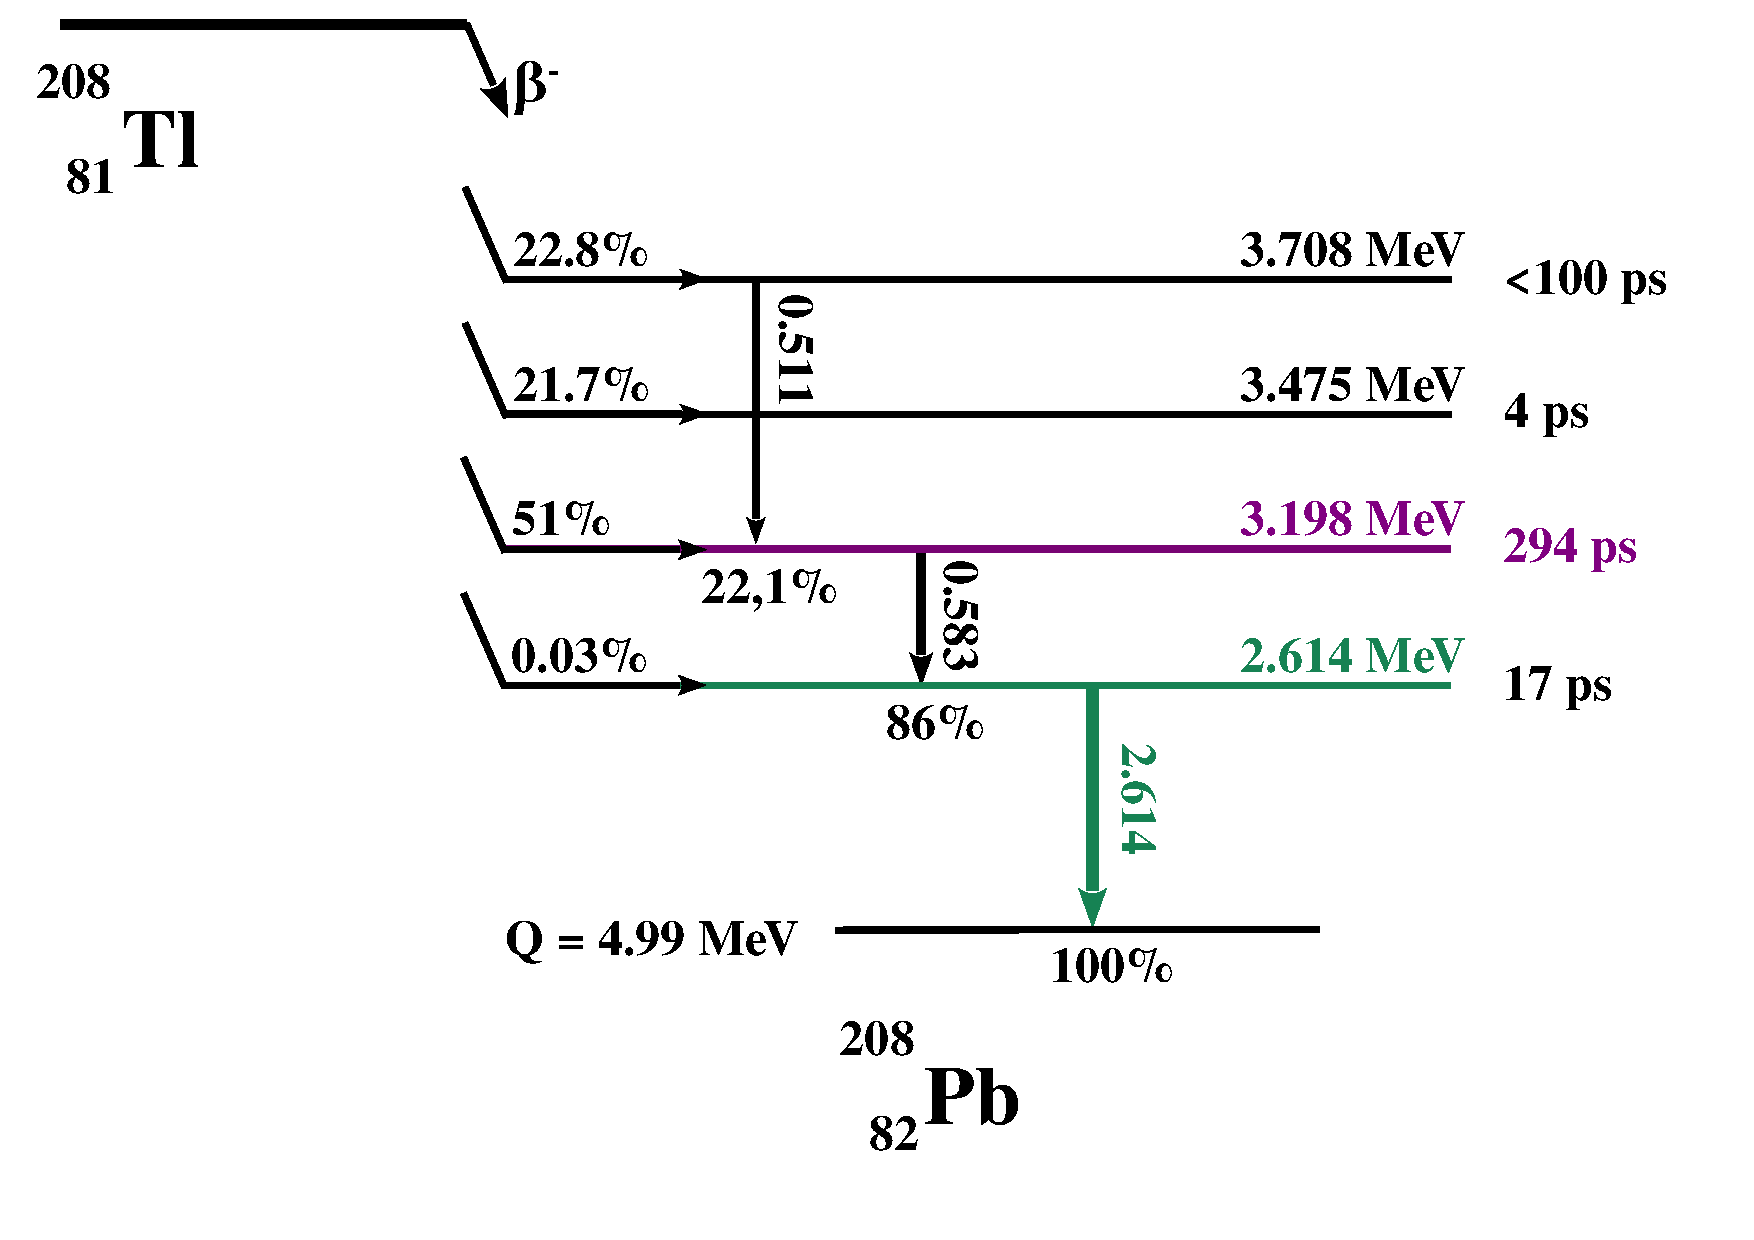
\includegraphics[width=13cm]{timedifference/fig_timediff/Tl_decay_scheme.pdf}
  \caption{A simplified disintegration scheme for the \Tl\ isotope.
    $81$~\% of the disintegration pass through the $294$~ps metastable energy level (orange).
    All disintegration go through the $2.615$~MeV energy level (green), where an orbital electron is ejected in $0.246$~\% of the cases through the internal conversion process.
  \label{fig:Tl_scheme}}
\end{figure}
This shows that \Tl\ always $\beta$-decays to an excited state of the \Pb\ daughter nuclei.
In more than $99$~\% of the decays, at least 2 $\gamma$'s are expected after the $\beta$ emission.
For $\zeronu$ detection of $\beta\beta$ isotopes with high $\Qbb$, the most dangerous mode of $\beta\beta$-like events production comes from the internal conversion of the $2.615$ MeV-$\gamma$, resulting in one electron with an energy of $2.5$ MeV approximately and a beta-electron with a continuous spectrum between $0$ and $\sim~1.5$~MeV.

\subsection{The internal conversion process}

An excited nucleus will practically constantly achieve a transition to a lower state by one of two processes: the emission of a $\gamma$-ray, or the ejection of one of the orbital electrons.
The latter, called \emph{internal conversion} (frequently abbreviated IC), is a second-order process, where one electron couples to one of the proton inside the excited nucleus.
Thus, in such a radioactive decay, the de-excitation energy of the nucleus is transferred \emph{directly} to a $j$-shell electron ($j=K,L,M...$).
A high-energy electron is therefore emitted from the atom, and carry off the energy
\begin{equation}
E_{IC} = E_{\gamma}-E_{j}\qquad (j=K,L,M...)\,,
\end{equation}
where $E_{j}$ is the binding energy of the electron in the $j$-shell, and $E_{\gamma}$ is the energy of the $\gamma$-ray.

This mechanism is possible because there is a non-zero probability of finding the electron within the nucleus, that is to say, the wave-function of the electron can penetrate the volume of the nucleus.
Consequently, due to their high nuclear penetration, electrons coming from the $1s$ state are more likely to be ejected (this transition is called $K$ internal conversion).
Although electrons coming from $2s$, $3s$ and $4s$ states ($L$, $M$ or $N$ internal conversions) have also a non-zero probability to undergo this process.
After the electron ejection, the hole in the corresponding shell is filled by an electron from a higher energy level, emitting characteristic $X$-rays, Auger electrons, or both.

For a given transition, the internal conversion coefficient of the electron in the $j$-shell, is defined by
\begin{equation}
\alpha_{j}=\frac{P_{IC, j}}{P_{\gamma}}\,,
\end{equation}
%% \begin{equation}
%% \alpha_{K}=\frac{P_{IC, K}}{P_{\gamma}}\,,
%% \end{equation}
where $P_{IC,j}$ is the $j$ conversion electron emission probability, and $P_{\gamma}$ is the $\gamma$-ray emission probability.
The total coefficient is
\begin{equation}
  \alpha_{T}=\sum_{j=K,L,M\cdots}\alpha_{j}\,.
\end{equation}
These coefficients are given in Tab.~\ref{tab:IC_prob} for the $2.615$~MeV energy level of \Tl\ isotope.
\begin{table}[!h]
  \centering
  \begin{tabular}{|c|c|c|c|c|}
    \hline
    Emission probability (\%) & $\alpha_{K}$ (\%) & $\alpha_{L}$ (\%) & $\alpha_{M}$ (\%) & $\alpha_{T}$ (\%) \\
    \hline\hline
    $100$ & $0.1708$ &    $0.0292$ &  $0.00685$  &    $0.246$ \\
    \hline
  \end{tabular}
  \caption{Internal conversion coefficients for the $2.615$~MeV $\gamma$-ray of the \Tl\ decay scheme.
    \label{tab:IC_prob}}
\end{table}
Therefore, in $0.246$~\% of the cases, the \Pb\ excited nucleus will undergone an internal conversion corresponding to the $2.615$~MeV energy level.


\subsection{\Tl\ disintegrations in the 2e channel}

Finally, a \Tl\ decay can present a two-electrons topology when, after the $\beta$ emission, an electron is ejected from the atom through internal conversion.
Especially, when this energy transfer corresponds to the $2.615$~MeV $\gamma$-ray, the ejected electron carry off a significant energy, depending on its initial binding energy with the nucleus.
For instance an orbital electron from the $K$-shell is ejected with an energy $E_{IC,K}=2.526$~MeV (${\alpha_{K}=0.17}$\%).
This decay is therefore likely to contribute in the region of interest for the $\zeronu$ search of \Se, or even \Nd.
In Fig.~\ref{fig:Emin_Emax_Tl} is presented the individual energy spectra for $2e$ topologies for \Tl\ simulations inside the source foils.
\begin{figure}[!h]
  \centering
  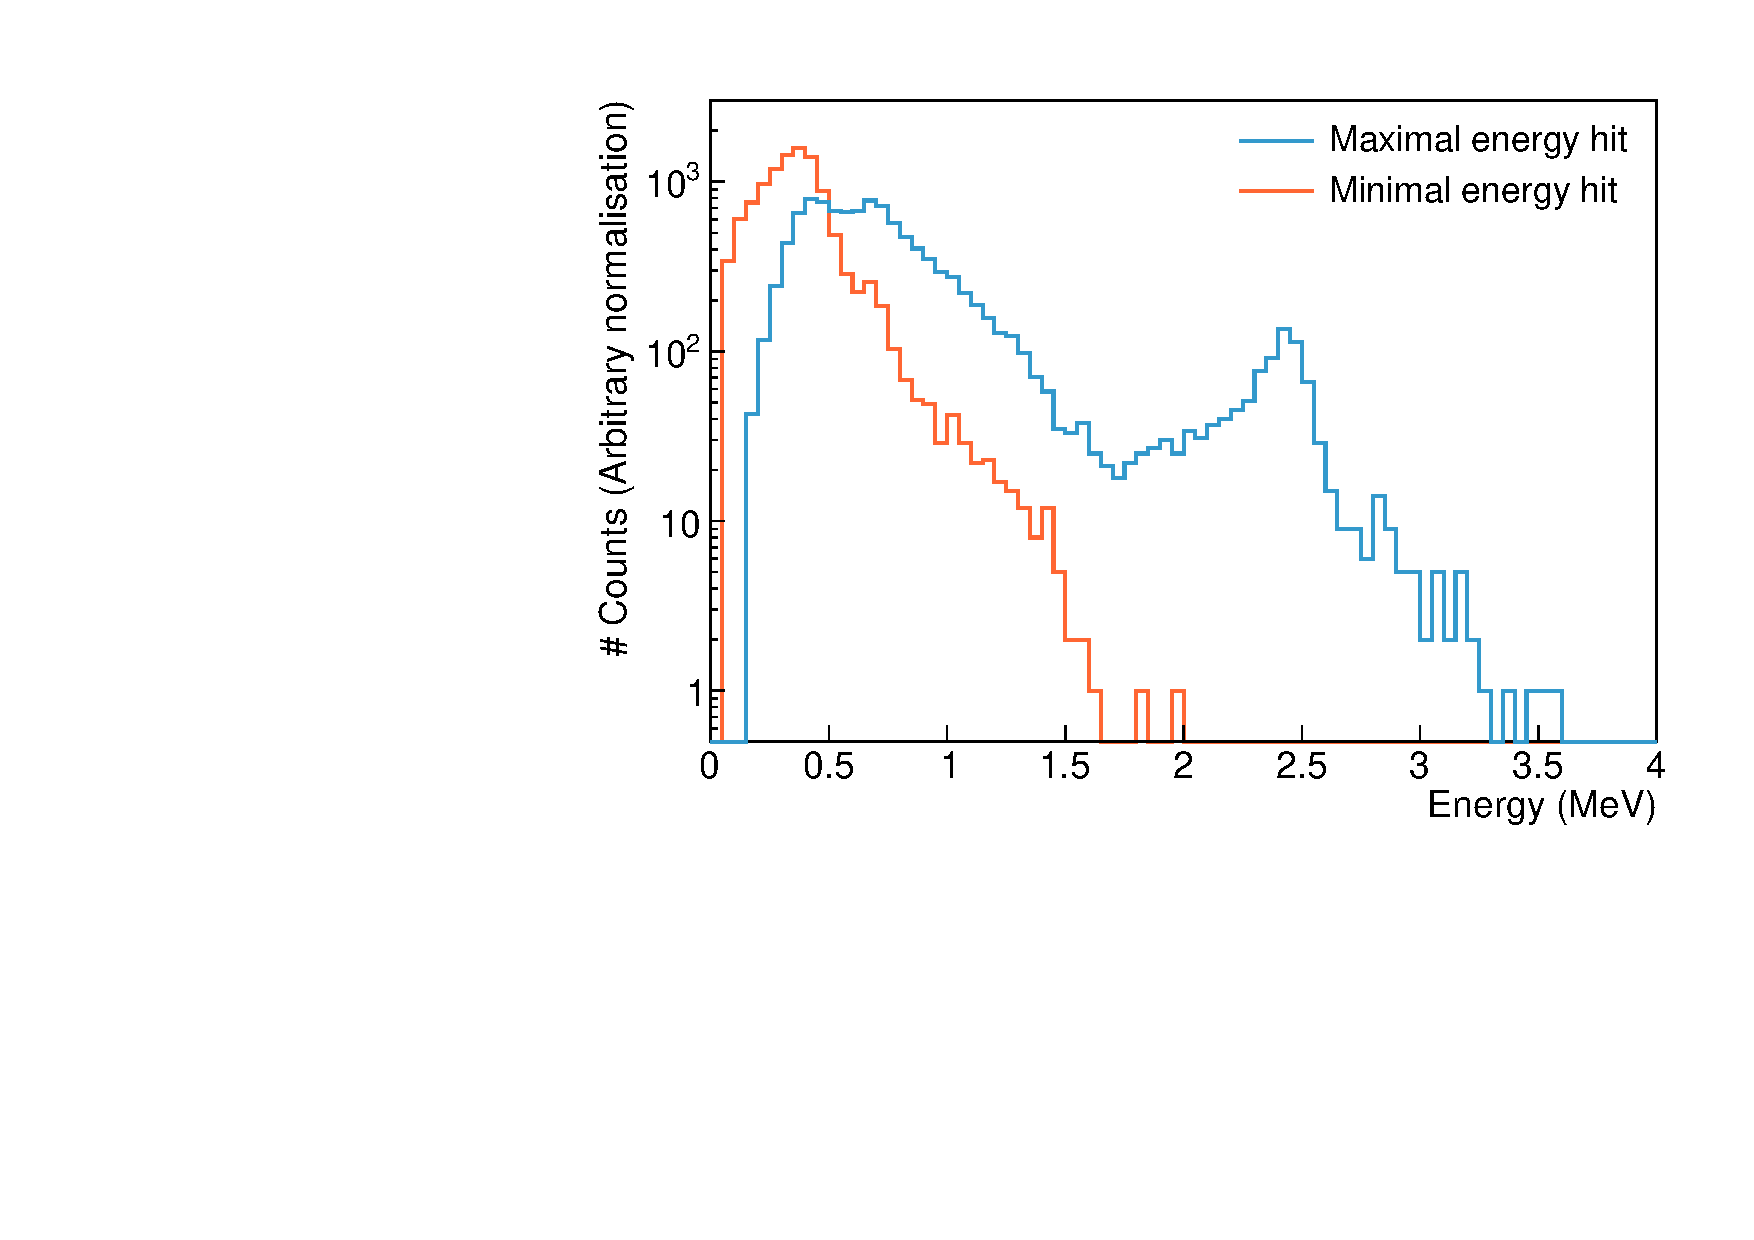
\includegraphics[width=13cm]{timedifference/fig_timediff/energy_spect_min_max_208Tl.pdf}
  \caption{Individual energy spectra for selected $2e$ topologies of \Tl\ decays simulated inside the source foils.
    Calorimeter hit of minimal energy (red) and maximal energy (blue).
    Spectra are arbitrarily normalised.
    The [$2.7$;$3.2$] ROI is represented by grey dashed lines.
    \label{fig:Emin_Emax_Tl}}
\end{figure}

An usual technique to reject \Tl\ background consists in distinguishing $2e$ topologies for which one of the two calorimeter hit has an energy greater than $2.7$~MeV.
The energy resolution of the demonstrator being improved by a factor of $\sim~2$ with respect to NEMO-$3$, this selection is efficient.
This cut-off allows to reject $0.61$~\% of the \Tl\ internal events, while rejecting only $0.11$~\% of $\zeronu$ events.

In the $2e$ channel, optimised topological cut-offs, based on time-of-flight computation and the distance between vertices, were presented in the previous chapter.
They are mostly efficient in rejecting the non-internal \Rn\ events.
In the next section, we remind and precise the internal probability computation, and present a new selection, also based on the time-of-flight computation, to reject the \Tl\ background.

\begin{itemize}
\item donner la proportion d'ev retardés avec la bank SD (simus en train de tourner)
\item relire et compléter cette sous-section
\end{itemize}

\section{Rejection of \Tl\ with a time-of-flight criterion}
\label{sec:Tl_TOF}

\begin{itemize}
\item Un des deux gamma est retardé de 294 ps, puis conversion interne -> donner la proportion de retardés (nb d'ev attendus, dans la ROI)
\item Avant d'entrer dans le détail préciser le principe de la réjection par temps de vol.
  L'électron de plus haute énergie est en retard, avec un retard en moyenne de 294 ps pour la plupart des niveaux (discuter un peu le schéma de désintégration, dans quel cas il sera en retard).
  Ensuite dire que tu as quantifié le pourcentage d'électrons de haute énergie en retard avec une simulation "parfaite" i.e. avec une résolution en  temps  nulle.
  A comparer avec le chiffre donné précédemment (issu d'une étude du schéma de désintégration.)
\item parler ici des simus avec sigma t nul, et du fait qu'on fait varier ce paramètre après coup dans l'analyse : même faire une sous partie
\item dire d'ailleurs qu'on utilise le PID, notamment pour le calcul de Pint
\end{itemize}

%% Internal conversion occurs after $\beta$ or $\alpha$ radioactive decays leaving the nucleus excited.
%% Then a $\gamma$ particle is emitted and transfers its energy to an atomic electron which results in ejection of this electron from the atom.
%% The emitted electron has an energy corresponding to the energy of previously excited nucleus reduced by the electron binding energy.
%% After the internal conversion, electrons reorganise.
%% The hole in internal layer is filled by an electron from an external layer (emitting an X ray).\\
%% The probability for an atomic electron to be ejected decreases with the initial binding energy.
%% Thus, electrons from K layers have a higher probability to be converted (see Fig.~\ref{fig:Tl_IC}).

\subsection{The internal probability}

The internal probability is a tool used to reject non-simultaneous events and is presented in detail in Chapter~\ref{ch:detector}.
As part of the analysis pipeline, it is widely employed in NEMO-$3$ and SuperNEMO, for background rejection purposes.
We examine an example of its usefulness in Chapter~\ref{ch:sensitivity}.
Nevertheless, for reasons to be given latter, in the current chapter, we need to perform our own calculation of internal probability, after the reconstruction pipeline.
That is an opportunity to come back to this tool and to clarify certain points.

The calculation of the internal $\chi^{2}$ is reminded in Eq.~\eqref{eq:int_chi2_electrons}, for two detected electrons, as a function of the expected time-of-flights, $t^{\text{exp}}$, the experimentally measured time-of-flights, $t^{\text{meas}}$, as well as the total uncertainty on the time-of-flight measurement:
\begin{equation}
  \chi^{2}_{int}=\frac{((t^{\text{meas}}_{1} - t^{\text{exp}}_{1}) - (t^{\text{meas}}_{2} - t^{\text{exp}}_{2}))^{2}}{\sigma_{t_{1}}^{2}+\sigma_{t_{2}}^{2}+\sigma_{\beta_{2}}^{2}+\sigma_{\beta_{1}}^{2}+\sigma_{l_{1}}^{2}+\sigma_{l_{2}}^{2}}\,,
  \label{eq:int_chi2_electrons}
\end{equation}
where $\sigma_{t_{i}}$ is the uncertainty on the measured time-of-flight of the particle $i$.
$\sigma_{\beta_{i}}$ and $\sigma_{l_{i}}$ are the uncertainties on the expected time-of-flight brought by the uncertainty on particle energies and track lenghts, respectively.
In the official SuperNEMO reconstruction pipeline, the latter is set up to ${\sigma_{l}=\sigma_{l_{1}}=\sigma_{l_{2}}=70}$~ps for electron particles.
As, therein chapter, we are focusing on two-electrons channels, we would check that the value of this parameter is correctly evaluated.

\subsubsection*{Optimisation of $\sigma_{l}$}

One way to examine if $\sigma_{l}$ is well-evaluated is to look at the flatness of the internal probability distribution for $\zeronu$ events in the $2e$ topology, for which a flat distribution is expected.
Indeed, the slope of this distribution provides pertinent information to check the estimation of uncertainties.
The flatter the distribution, the more correctly uncertainties are estimated.

Discret values of $\sigma_{l}$ running from $0.01$ to $0.1$~ns are used to compute internal probability ditributions for $\zeronu$ decays simulations inside the source foils.
We select merely $2e$ topologies by using the first order cuts, presented in Chapter~\ref{ch:sensitivity}, such that the internal hypothesis is almost certain to be verified.
For each distribution, a linear fit is performed on the reduced range \Pint$~\in[0.1;1]$ in order to avoid the peak at low internal probabilities.
The \emph{flatness parameter} $a_{F}$ is defined as the slope parameter of the linear fit.
The optimisation then consists in finding the value of $\sigma_{l}$ for which the parameter $a_{F}$ is cancelled, which corresponds to the best estimate for $\sigma_{l}$.

In Fig.~\ref{fig:flatness} is given the slope $a_{F}$ as a function of $\sigma_{l}$.
\begin{figure}[!h]
  \centering
  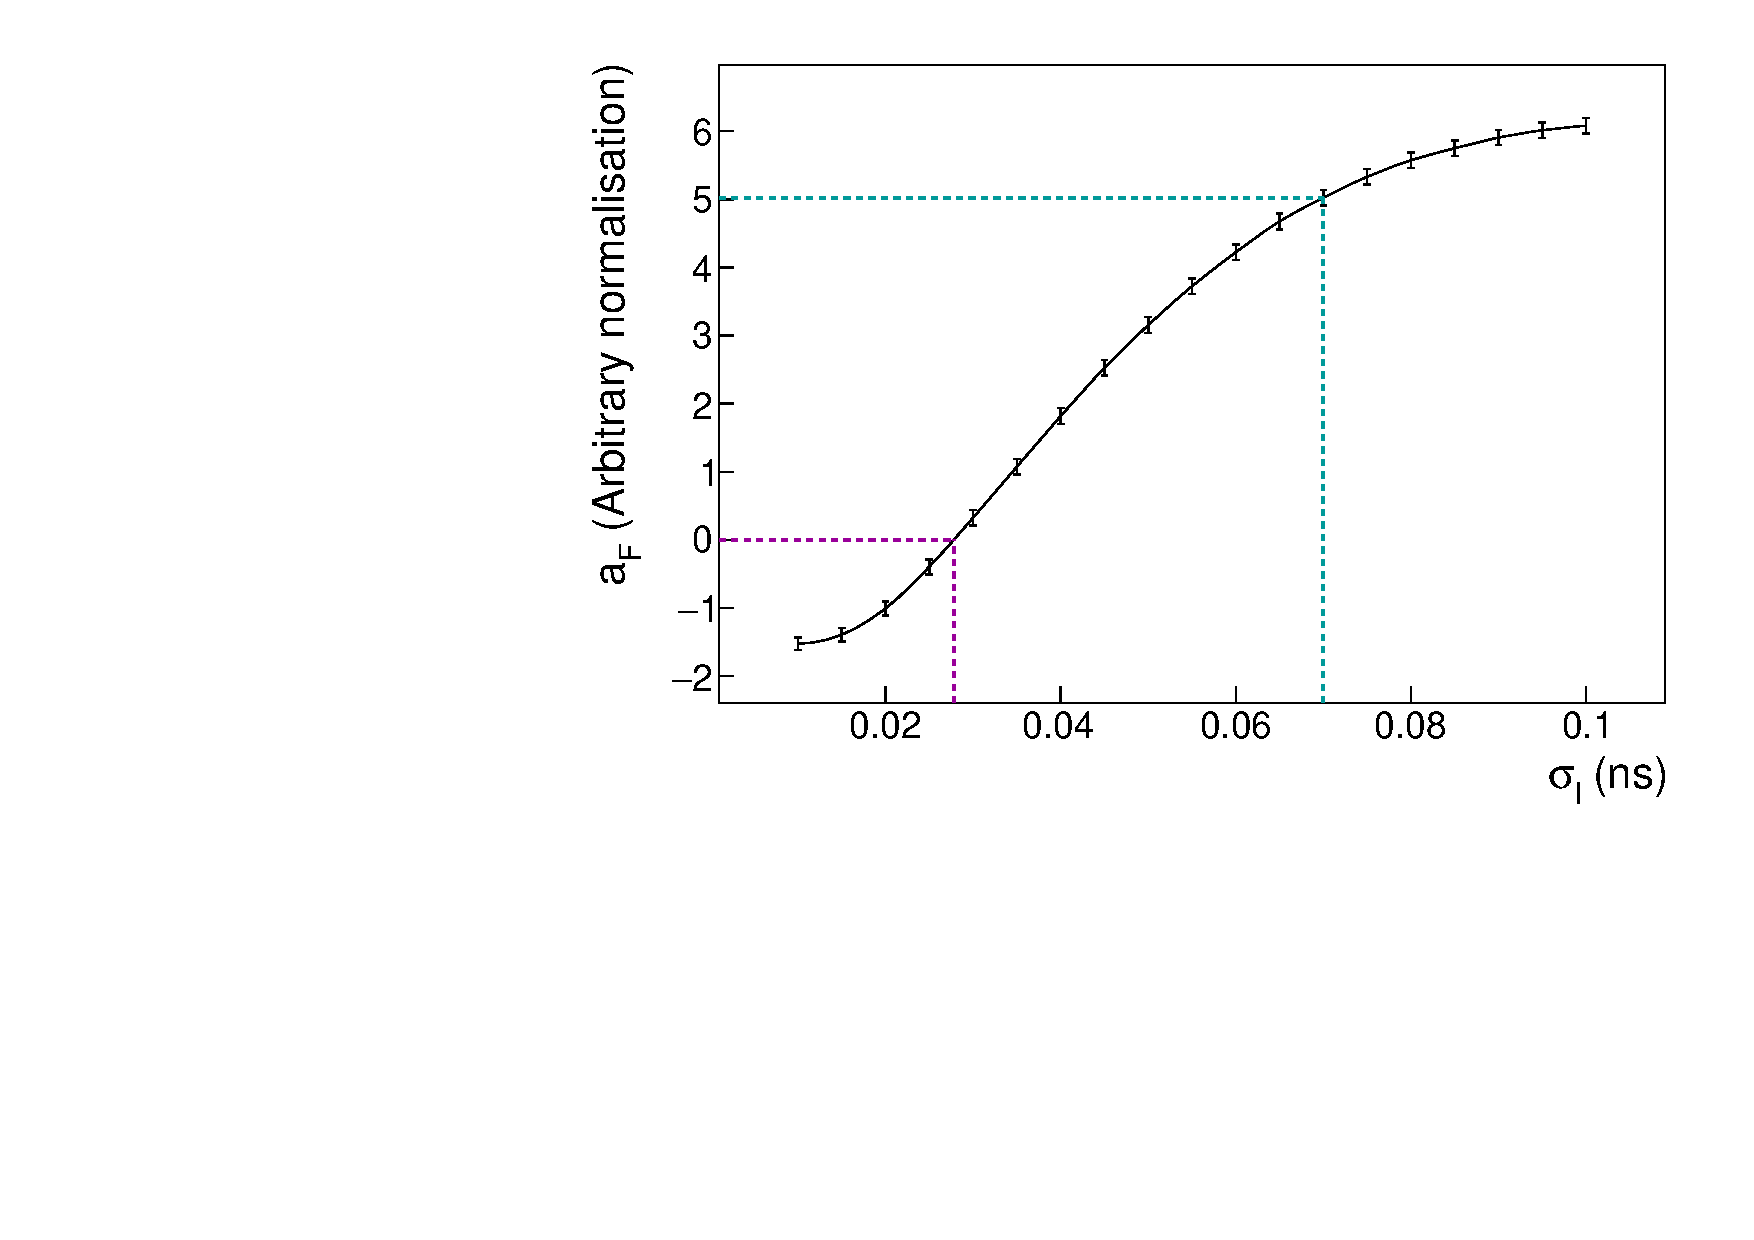
\includegraphics[width=13cm]{timedifference/fig_timediff/flatness.pdf}
  \caption{Slope $a_{F}$ as a function of the time uncertainty due to the reconstructed track length $\sigma_{l}$.
    The former value used in the SuperNEMO reconstruction pipeline is pointed out by blue dashed lines.
    The value kept for $\sigma_{l}$ is the one for which $a_{F}=0$, $\sigma_{l}~=~27.8~\pm~0.8$~ps, showed by purple dashed lines.
    The errors made on the $a_{F}$ fit parameter are represented by the grey filled area.
    \Pint\ is calculated for $\zeronu$ decays simulated inside the source foil, with first order cut-offs applied.
    \label{fig:flatness}}
\end{figure}
For $\sigma_{l}=70$~ps, $a_{F}>0$, revealing an overestimation of uncertainties in the computation of the internal $\chi^{2}$ in the SuperNEMO reconstruction pipeline, at the Particle Identification module level.
The optimised value, kept for the further analysis, is $\sigma_{l}~=~27.8~\pm~0.8$~ps.
In Fig.~\ref{fig:Pint_comparison} is displayed the internal probability distributions for these two values of the $\sigma_{l}$ parameter, $\sigma_{l}=70$~ps and $\sigma_{l}=27.8$~ps.
\begin{figure}[!h]
  \centering
  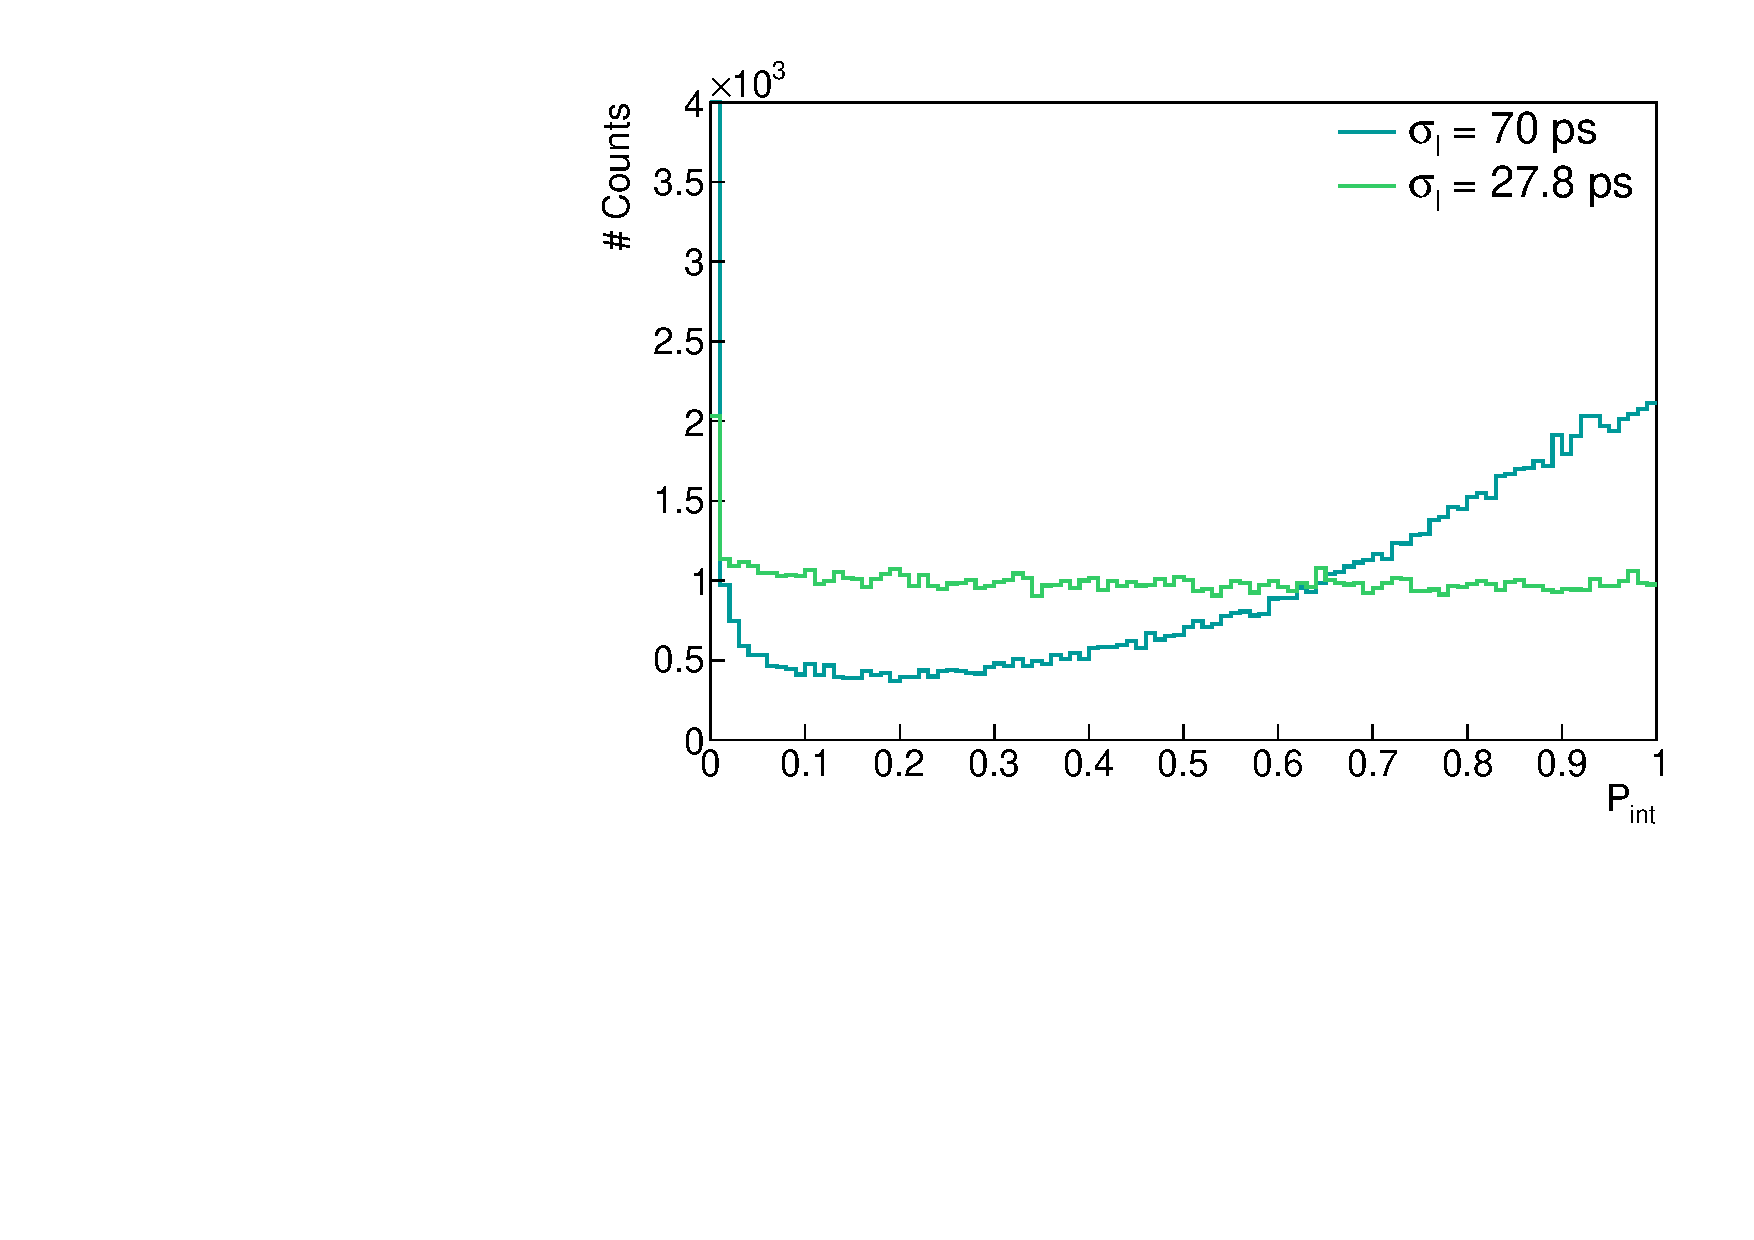
\includegraphics[width=13cm]{timedifference/fig_timediff/Pint_comparison.pdf}
  \caption{Internal probability distributions for $\sigma_{l}=70$~ps (blue) and $\sigma_{l}=27.8$~ps (green).
    \Pint\ is calculated for $\zeronu$ decays simulated inside the source foil, with first order cut-offs applied.
    \label{fig:Pint_comparison}}
\end{figure}
Let us notice that normally $\sigma_{l}$ should depend on the track length as well as the energy, especially as multiple scatterings in the tracker have a more notable impact for low energy electrons.
A more complete analysis would then compare the simulated track lengths with the reconstructed ones, for different energy simulated sets of mono-kinetic electrons, to evaluate this dependence.
Nevertheless, our optimisation is good enough for the current analysis.
We use this optimisation for the rest of this analysis, and discussion is in progress to modify this parameter in the SuperNEMO software.

The internal probability is principally designed to reject non-simultaneous events coming from the source foils.
Therefore, it is extremely effective in rejecting \Rn\ events produced far from the source foils.
Even if it is less, this criterion is also effective in rejecting \Tl\ events due to the metastable state of the $2.615$~MeV-$\gamma$.
But to describe even better these internal conversion events we would set up a new law of probability that would express the hypothesis that a given event is from a $\beta$+IC delayed \Tl\ disintegration.

\subsection{The exponential probability for \Tl\ events}

According to the disintegration scheme of the \Tl\ isotope (Fig.~\ref{fig:Tl_scheme}), there is an $81~\%$ probability of passing through the $294~$ps metastable level.
After that, to attain the ground state of \Pb, the excited nucleus has $100\%$ of probability to decay through the $2.615$ MeV energy level.
At this occasion, in $0.246\%$ of cases (Tab.~\ref{tab:IC_prob}), one of the orbital electrons is ejected from the atom following the internal conversion process.
To summarise, for $0.20$~\% of the total \Tl\ decays, a $\beta$ particle is emitted, and a delayed orbital electron is ejected through internal conversion of the $2.6$ MeV-$\gamma$.
Furthermore, $X$\% of the events with an energy sum greater than $2.7$~MeV (the ROI low bound) are from delayed internal conversion decays.
We aim to use this delayed electron to discriminate \Tl\ internal background from the $\zeronu$ signal.

\begin{itemize}
\item relire cette partie quand les simus sont finies
\end{itemize}

\subsubsection{Probability density function}

For a given detected $2e$ topology, we define the $\Delta t^{meas}$ parameter as
\begin{equation}
  \Delta t^{meas} = t_{1}^{meas}-t_{2}^{meas}\,,
  \label{eq:time_diff}
\end{equation}
where $t_{1}^{meas}$ and $t_{2}^{meas}$ are the two measured time-of-flights, with $t_{2}$ for the electron of lowest energy, and $t_{1}$ for the one of highest energy.
If this $2e$ topology corresponds to a delayed \Tl\ event, then the electron of lowest energy is supposed to be a $\beta$ particle and the one of highest energy an electron coming from an internal conversion.
Assuming an ideal calorimeter perfectly measuring time-of-flights and energies, the $\Delta t$ distribution for such delayed events would be a decreasing exponential, with the decay parameter ${\tau=294}$~ps.
However, in actual conditions, this exponential is degraded by the uncertainties on time-of-flight measurements detailed in Eq.~\eqref{eq:int_chi2_electrons}.
These are embedded by a Gaussian distribution centred around ${\mu=0}$~ps with a given width $\sigma$.
Therefore, to each $2e$ topology is associated a probability density function which is the convolution between an exponential and a Gaussian distribution, written down as ${(E \otimes G)_{\tau,\mu,\sigma}(\Delta t)}$.
The corresponding value of $\Delta t^{meas}$ is then found somewhere on this distribution, and will serve us to define the so-called \emph{exponential probability}, $P_{exp}(\Delta t^{meas})$, which is the probability that this event comes from a $\beta$+IC delayed decay.

\begin{itemize}
\item Du coup mettre une distribution de ces ev sur l'exponentielle
\end{itemize}

\subsubsection{Exponential probability}

We wish to define this probability following the same principle as for the internal probability, for comparison purposes.
Therefore, we would obtain the maximal value ${P_{exp}=1}$ when the value of $\Delta t$ is the most favourable, i.e. when $\Delta t$ is of the order of the mean of the ${(E \otimes G)_{\tau,\mu,\sigma}(\Delta t)}$ distribution.
On the other hand, minimal values for $P_{exp}$ would be reached for unfavourable values of $\Delta t$, so ${P_{exp} \xrightarrow[|\Delta t| \rightarrow +\infty]{} 0}$.
To do so, the ${(E \otimes G)_{\tau,\mu,\sigma}(\Delta t)}$ distribution is normalised and the exponential probability is defined as
\begin{equation}
  P_{exp}(\Delta t^{meas}) = \int_{-\infty}^{\Delta t^{meas}} (E \otimes G)_{\tau,\mu,\sigma}(t)\, dt + \int_{\Delta t_{sym}^{meas}}^{-\infty} (E \otimes G)_{\tau,\mu,\sigma}(t)\, dt\,,
  \label{eq:Pexp}
\end{equation}
where $\Delta t^{meas}_{sym}$ is defined according to $\Delta t^{meas}$ of which a graphical representation is given in Fig.~\ref{fig:Pexp} to ease the explanation of its definition.
\begin{figure}[!h]
  \centering
  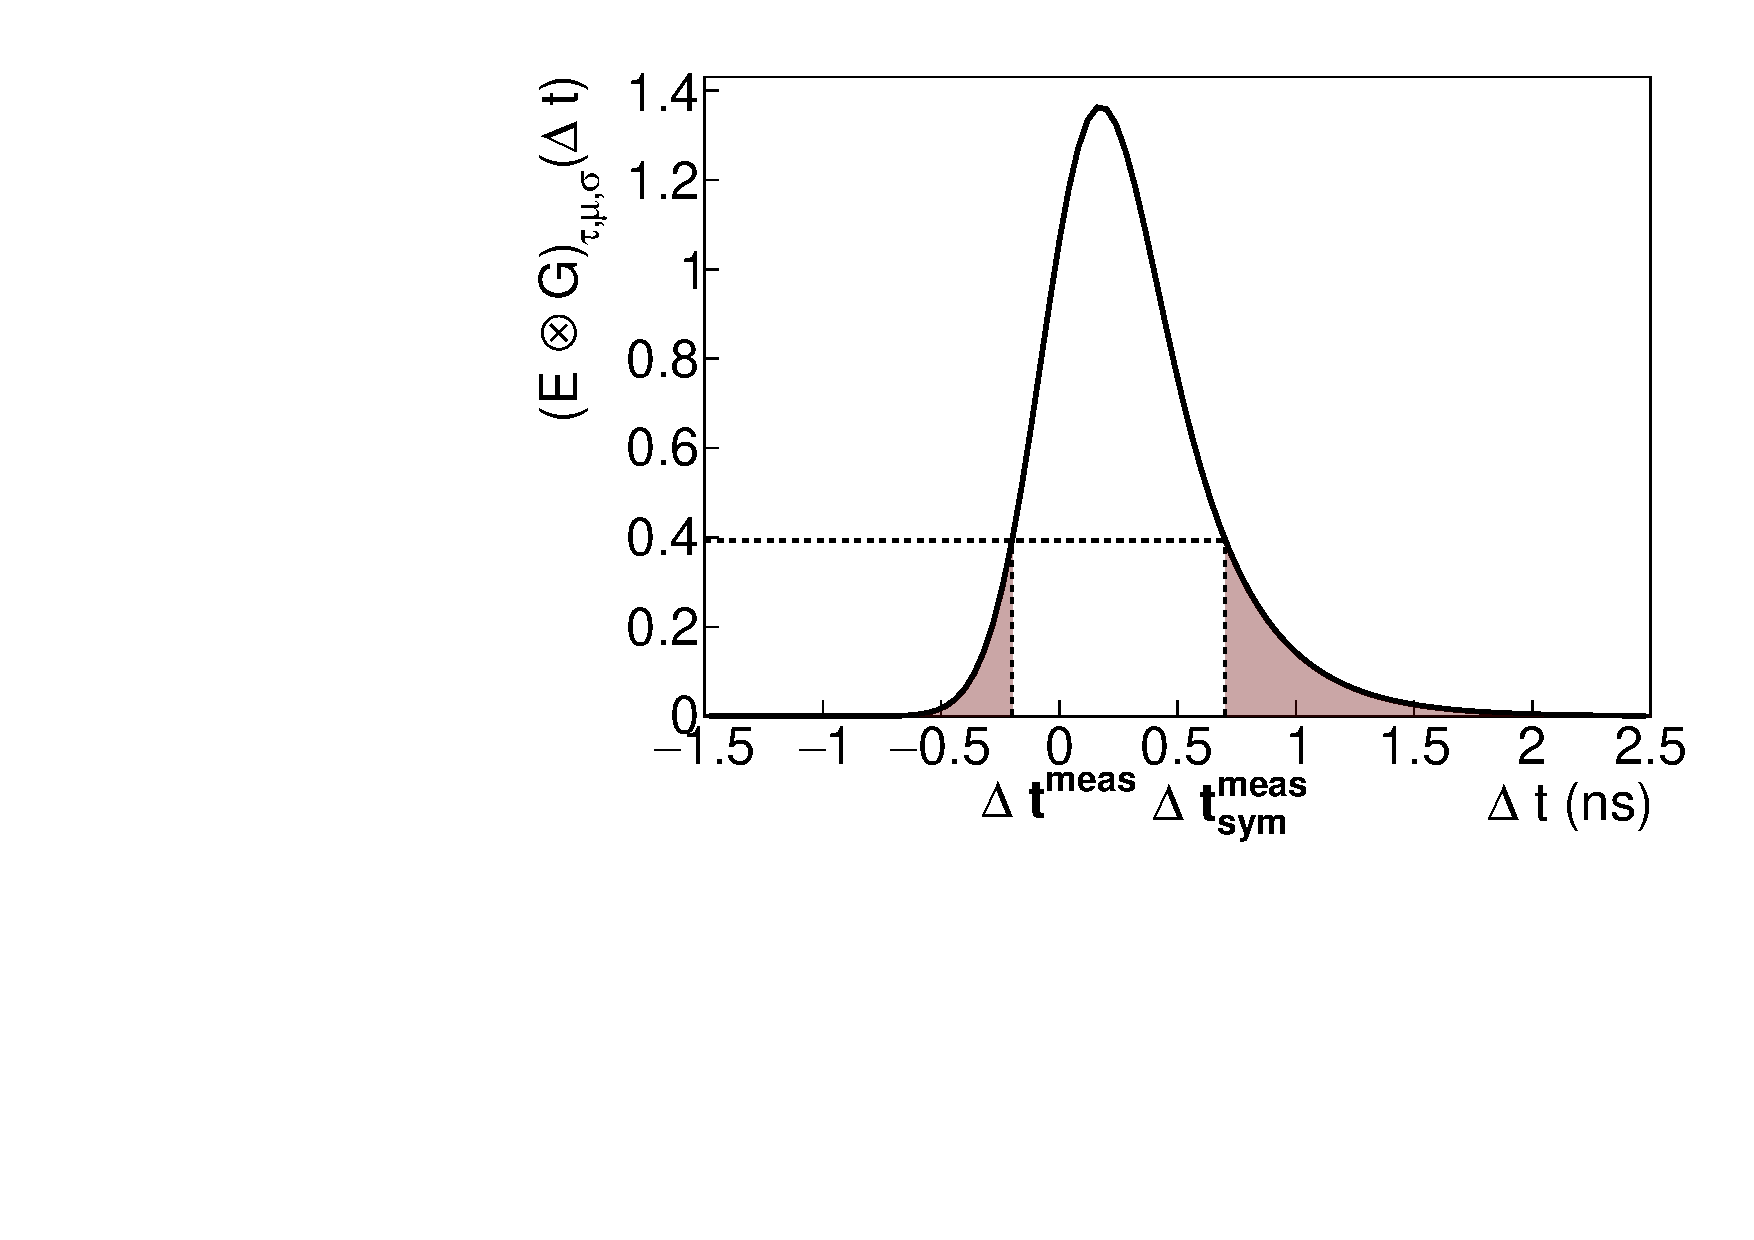
\includegraphics[width=13cm]{timedifference/fig_timediff/proba_expo_test.pdf}
  \caption{Normalised convolution distribution ${(E \otimes G)_{\tau,\mu,\sigma}(\Delta t)}$.
    The parameters are $\tau=294$~ps, $\mu=0$~ps and $\sigma=\sigma_{tot}$, computed with $\sigma_{l}=27.8$~ps and $\sigma_{t}=200$~ps.
    \label{fig:Pexp}}
\end{figure}
In this example the distribution corresponds to ${(E \otimes G)_{\tau,\mu,\sigma}(\Delta t)}$ with ${\tau=294}$~ps and ${\mu=0}$~ps and the total time uncertainty is calculated taking $\sigma_{l}=27.8$~ps and $\sigma_{t}=200$~ps.
The two integrals whose sum is given in the Eq.~\eqref{eq:Pexp} are represented by two red-coloured areas.
As explained, each probability density function is defined for a single $2$-electrons event.
Therefore, it depends on the value of the measured energies for the two particles detected.
In the given example, we considered two particles interacting inside the calorimeter with an energy of $1$~MeV each.

In fig.~\ref{fig:Pexp_Tl} are presented exponential probability distributions for $2e$ topologies selected of \Tl\ and $\zeronu$ simulations inside the source foils.
\begin{figure}[!h]
  \centering
  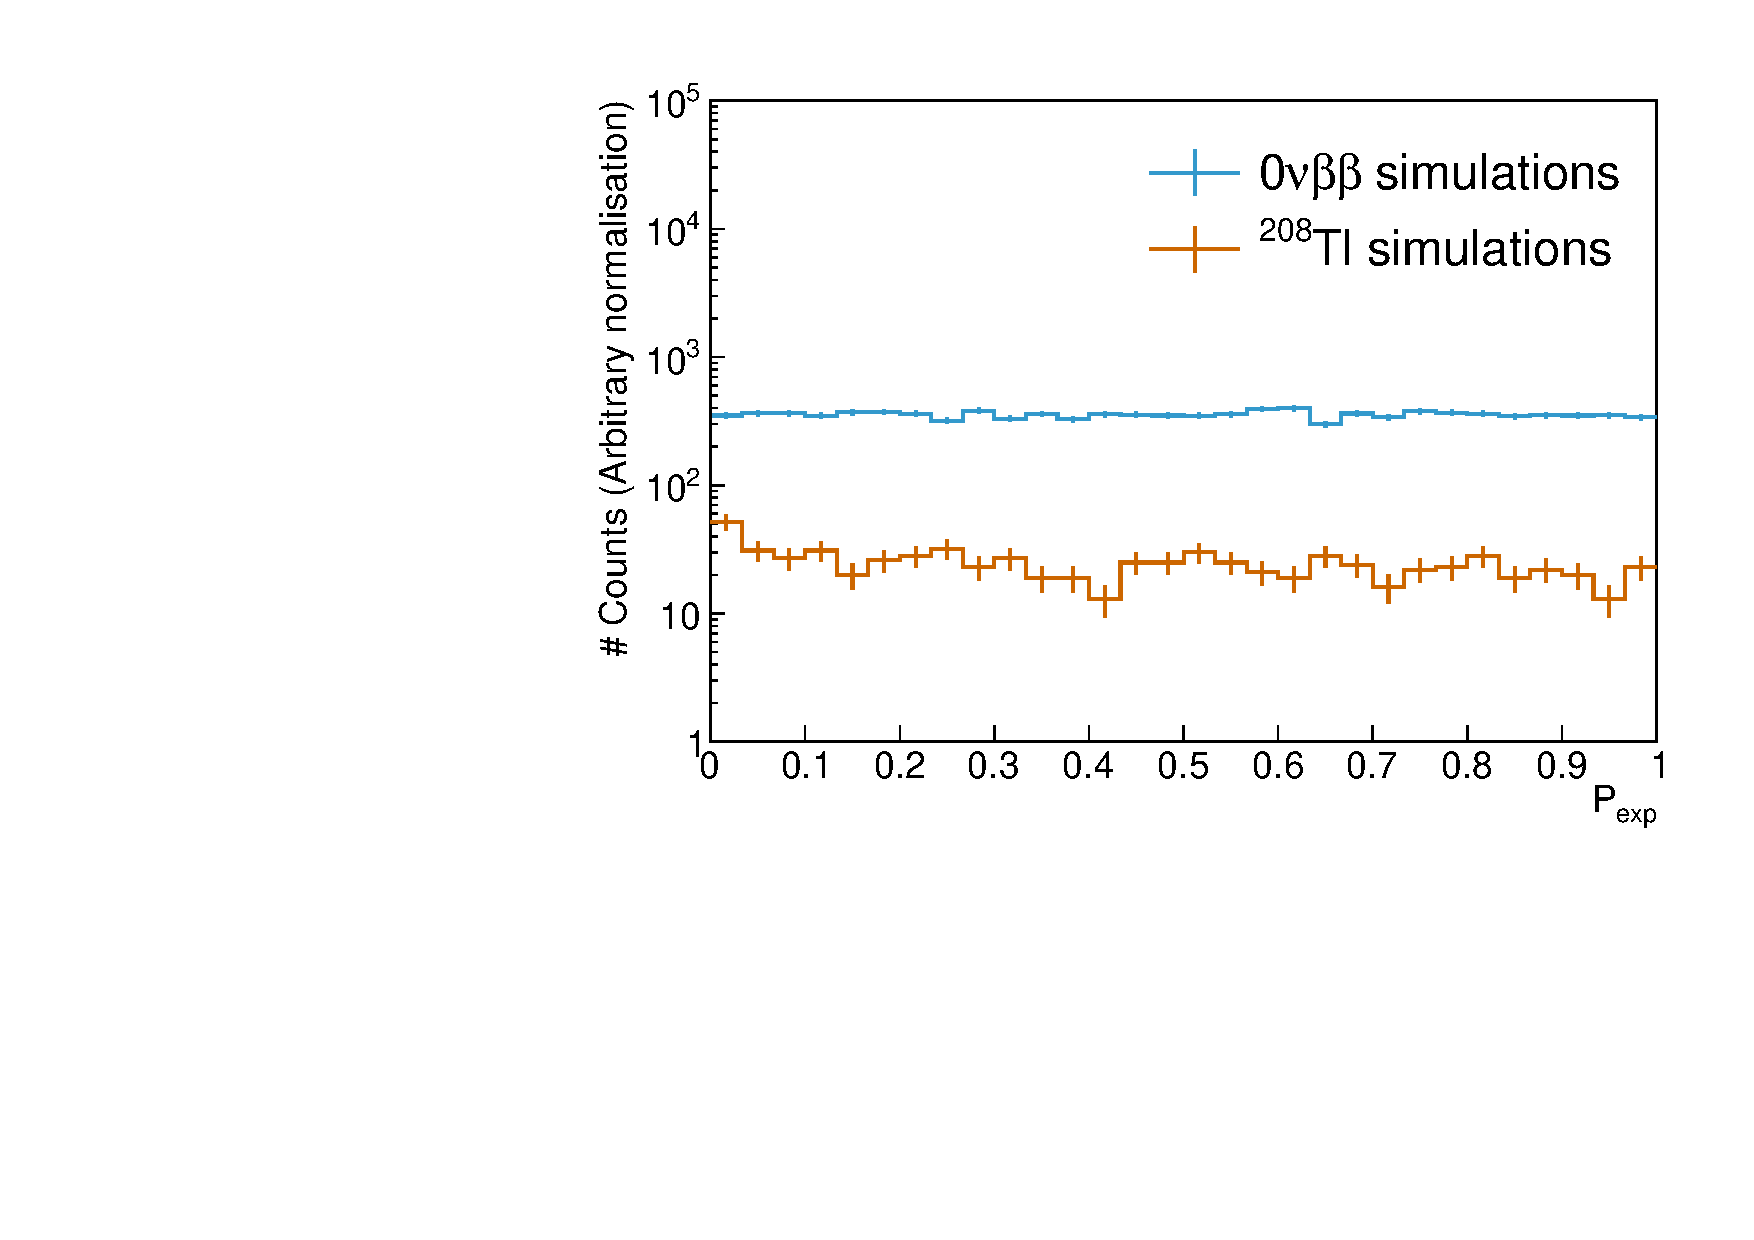
\includegraphics[width=13cm]{timedifference/fig_timediff/proba_expo_400.pdf}
  \caption{Exponential probability distribution for \Tl\ (orange) and $\zeronu$ simulations (blue), for $2e$ topologies with an electron energy sum greater than $2.7$~MeV (discussed in Sec.~\ref{sec:ev_selection}).
    $\sigma_{t}=200$~ps, $\sigma_{l}=27.8$~ps.
    \label{fig:Pexp_Tl}}
\end{figure}
As expected, the distribution is flat, since this probability was defined in the same way as the internal probability.
%%The distortion at low $P_{exp}$ comes from the proportion of events where the second electron doesn't come from the internal conversion of the $2.615$~MeV $\gamma$-ray.

Internal and exponential probabilities are two different tools based on particle time-of-flight measurements, adapted to describe internal and delayed events, respectively.

\section{Event selection}
\label{sec:ev_selection}


Now the exponential probability tool has been defined, the aim of this analysis is to set up events selections focusing on delayed \Tl\ events rejection.
Basic cut-offs are described, and compared with a more elaborated selection using these two probabilities.
The influence of the uncertainty $\sigma_{t}$ on time measurement is discussed at the end of the section.

\subsection{Energy selection}

Based on the conclusions given in the previous chapter, the lower bound of the region of interest optimising the search of $\zeronu$ decay stands at the electron energy sum of $2.7$~MeV.
From this energy, $2e$ topologies for \Tl\ are mainly populated by $\beta$ decays followed by the internal conversion of the $2.615$~MeV $\gamma$-ray.
In the following, we therefore focus only on events with a sum in energy of the two detected electrons greater than $2.7$~MeV.

\subsection{Time-of-flight cut-off}
\label{subsec:tof_cutoff}

Before using the two internal and exponential probabilities, a simple cut-off using the electron time-of-flight is explored.
Indeed, we are especially focused on rejecting the internal \Tl\ events for which the successive $\gamma$-rays emisions went through the $294$~ps half-life metastable state.
For these decays, we are expecting the particle of highest energy to be delayed compared with the one of lowest energy.
Each term in Eq.~\ref{eq:time_diff} corresponds to what it took for a particle to travel from the source to the calorimeter and depends on the time it spent in the source after emission, as well as how long it took to cross the tracker.
In order to remove from $\Delta t^{meas}$ the dependency on travel time in the tracker, we define the corrected time difference as
\begin{align}
  \Delta t^{\text{corr}} & = t^{\text{corr}}_{1} - t^{\text{corr}}_{2}\\
  & = (t^{\text{meas}}_{1} - t^{\text{exp}}_{1}) - (t^{\text{meas}}_{2} - t^{\text{exp}}_{2})\,,
\end{align}
where $t^{\text{corr}}_{i}$ are the corrected time-of-flights and $t^{\text{exp}}_{i}$ the expected ones calculated with the particle energy and track length (Eq.~\ref{eq:th_time}).

The two distributions $\Delta t^{meas}$ and $\Delta t^{\text{corr}}$ are presented in Fig.~\ref{fig:delta_t}, for $\zeronu$ and \Tl\ simulations inside the source foils.
\begin{figure}[!h]
\centering
\begin{subfigure}[t]{1.\textwidth}
  \centering
  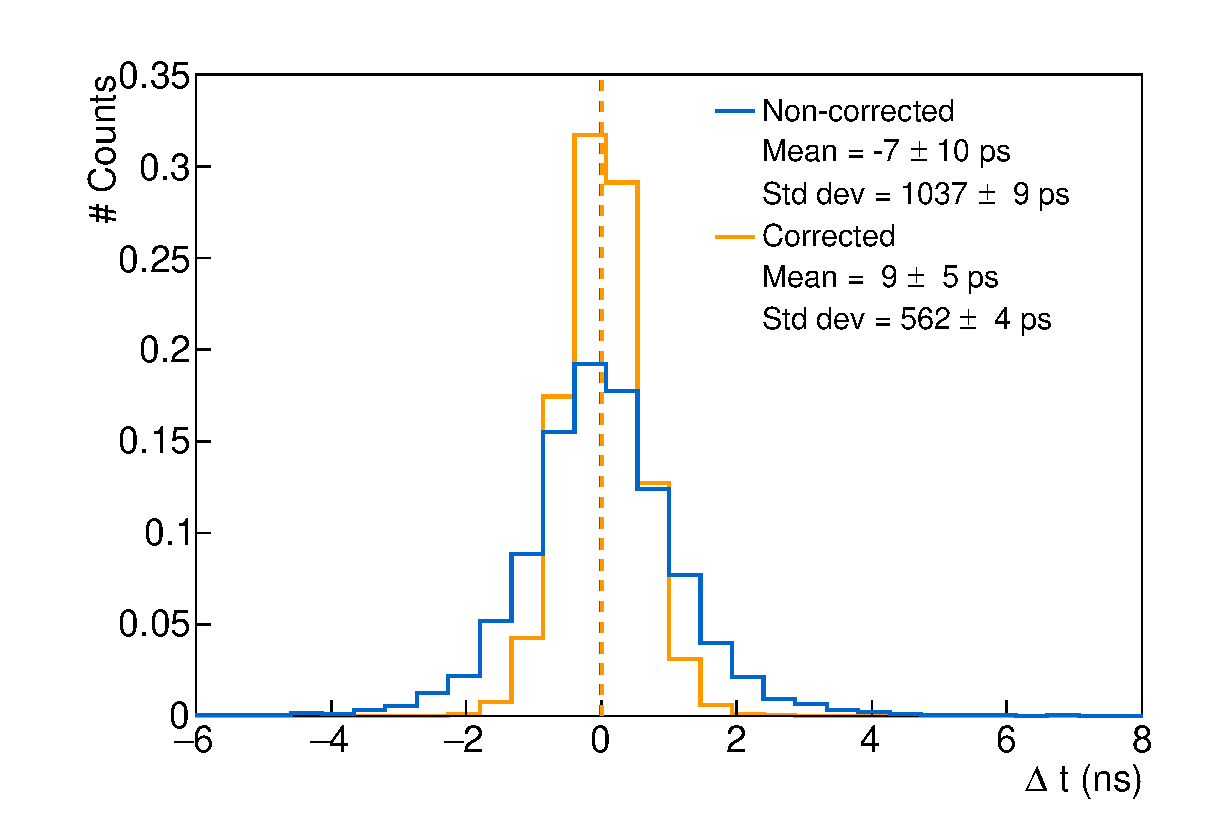
\includegraphics[width=0.7\textwidth]{timedifference/fig_timediff/0nubb_delta_t.eps}
  \captionsetup{justification=justified}
  \caption{$\zeronu$ simulations.
    \label{subfig:0nubb_delta_t}}
\end{subfigure}
\hfill
\begin{subfigure}[t]{1.\textwidth}
  \centering
  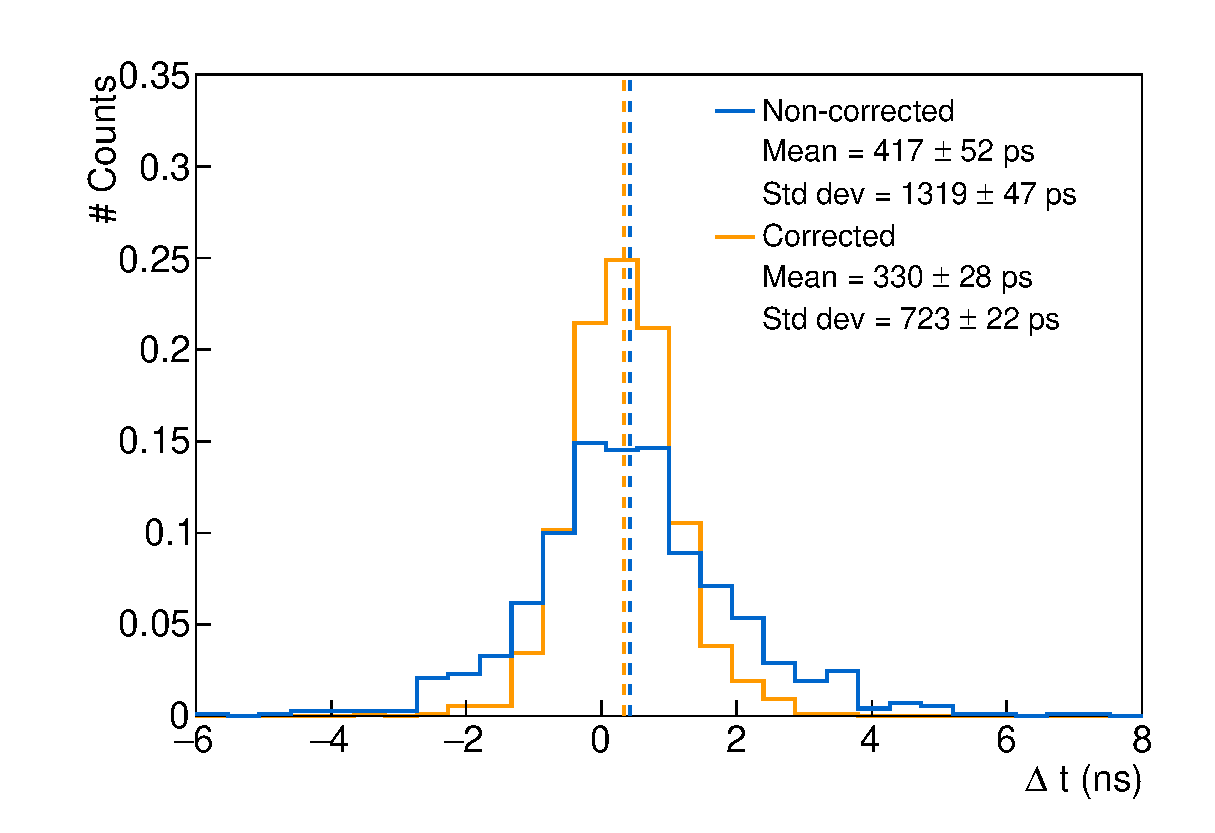
\includegraphics[width=0.7\textwidth]{timedifference/fig_timediff/208Tl_delta_t.eps}
  \captionsetup{justification=justified}
  \caption{\Tl\ simulations.
    \label{subfig:208Tl_delta_t}}
\end{subfigure}
\caption{Corrected (orange) and non-corrected (blue) time-of-flight difference between the two electrons.
  (a) $\zeronu$ simulations inside the source foils.
  (b) \Tl\ simulations inside the source foils.
  The first-order selections have been applied.
  The two distributions are normalised.
  $\sigma_{t}=200$~ps and $\sigma_{l}=27.8$~ps.
  \label{fig:delta_t}}
\end{figure}
For $\zeronu$ simulations, the $\Delta t^{corr}$ distribution is centred around zero, as the two electrons are expected to be emitted simultaneously.
Then, the correction on time difference only lowers the standard deviation of the distribution.
For \Tl\ simulations, the mean of the distribution is slightly shifted towards positive values.
Once corrected by the expected times, the mean difference between the two electrons time-of-flights stands at $330~\pm~28$~ps.
This is a direct consequence of the existence of $\beta$+IC delayed events, for which the particle of highest energy is expected to hit a calorimeter block at a time $t^{\text{corr}}_{1}~>~t^{\text{corr}}_{2}$.
Therefore, a simple way of rejecting the \Tl\ delayed events is to consider the sign of $\Delta t^{\text{corr}}$: these events are more likely to have $\Delta t^{\text{corr}}~>~0$.
A simple cut-off is to reject $2e$ topologies for which $\Delta t^{\text{corr}}~>~0$.

For a calorimeter time uncertainty of $\sigma_{t}~=~200$~ps, we are able to reject $76$~\% of \Tl\, while selecting $49$~\% of the $\zeronu$, for the $2e$ topologies with $E~>~2.7$~MeV.
Although we manage to reject a significant fraction of Thallium events, the impact of this cut is too high on $\zeronu$ events.
Moreover, the uncertainties on time-of-flights are not taken into account in the rejection criterion.
%%We study in Sec.~\ref{subsec:selection_optimisation} an optimization of this cut-off, including the influence of the temporal performance of the calorimeter $\sigma_{t}$.

\subsection{Probability cut-off}

At this level it is interesting to consider the internal and exponential probabilities to describe $2e$ topologies and attempt to obtain a higher background rejection.
They seem to be better tools notably because, unlike the $\Delta t^{\text{corr}}$ rejection criterion, they do take into account the time-of-flight uncertainties.
The first one was already used in Chapter~\ref{ch:sensitivity}, and is a widely-used tool to reject non-internal events.
The second was designed specifically for this analysis to identify delayed \Tl\ events, and also depends on the time of flight resolution through the convolution with a Gaussian function.

The idea is this section is to reject \Tl\ events taking into account their two values of internal and exponential probabilities.
Then it is interseting to represent them with a two-dimensional binned histogram of $P_{exp}$ as a function of \Pint, as done is Fig.~\ref{fig:biplot_Pexp_Pint}.
\begin{figure}[!h]
  \centering
  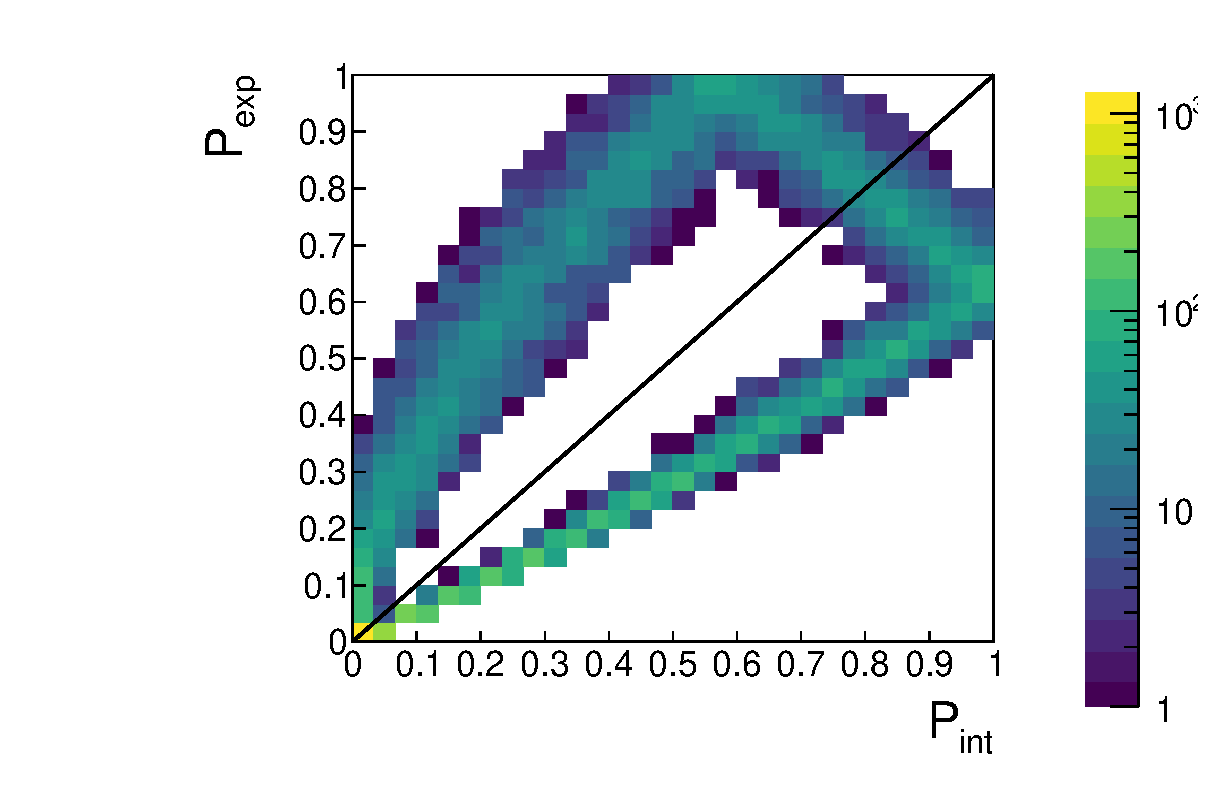
\includegraphics[width=15cm]{timedifference/fig_timediff/PintVSPexp_208Tl.eps}
  \caption{Two-dimensional histogram showing the $P_{exp}$ distribution as a function the \Pint\ distribution, for \Tl\ simulations.
    $\sigma_{t}=200$~ps and $\sigma_{l}=27.8$~ps.
    The first-order cut-off and the energy selection $>2.7$~MeV have been applied.
    \label{fig:biplot_Pexp_Pint}}
\end{figure}
In this particular example, we picture the variations of \Pint\ and $P_{exp}$ applying ${\sigma_{t}=200}$~ps, merely because it is interesting to see the distribution ${(E \otimes G)_{\tau,\mu,\sigma}(\Delta t)}$ with this value.
Nevertheless, we focus on the influence of this parameter later in Sec.~\ref{subsec:calo_sigma}.
We clearly distinguish three event populations in this histogram.
In order to better understand these variations, we give in Fig.~\ref{fig:proba_cut_ex} three examples of ${(E \otimes G)_{\tau,\mu,\sigma}(\Delta t)}$ distributions, each of them illustrating one of the three zones.
\begin{figure}[!h]
\centering
\begin{subfigure}[t]{0.95\textwidth}
  \centering
  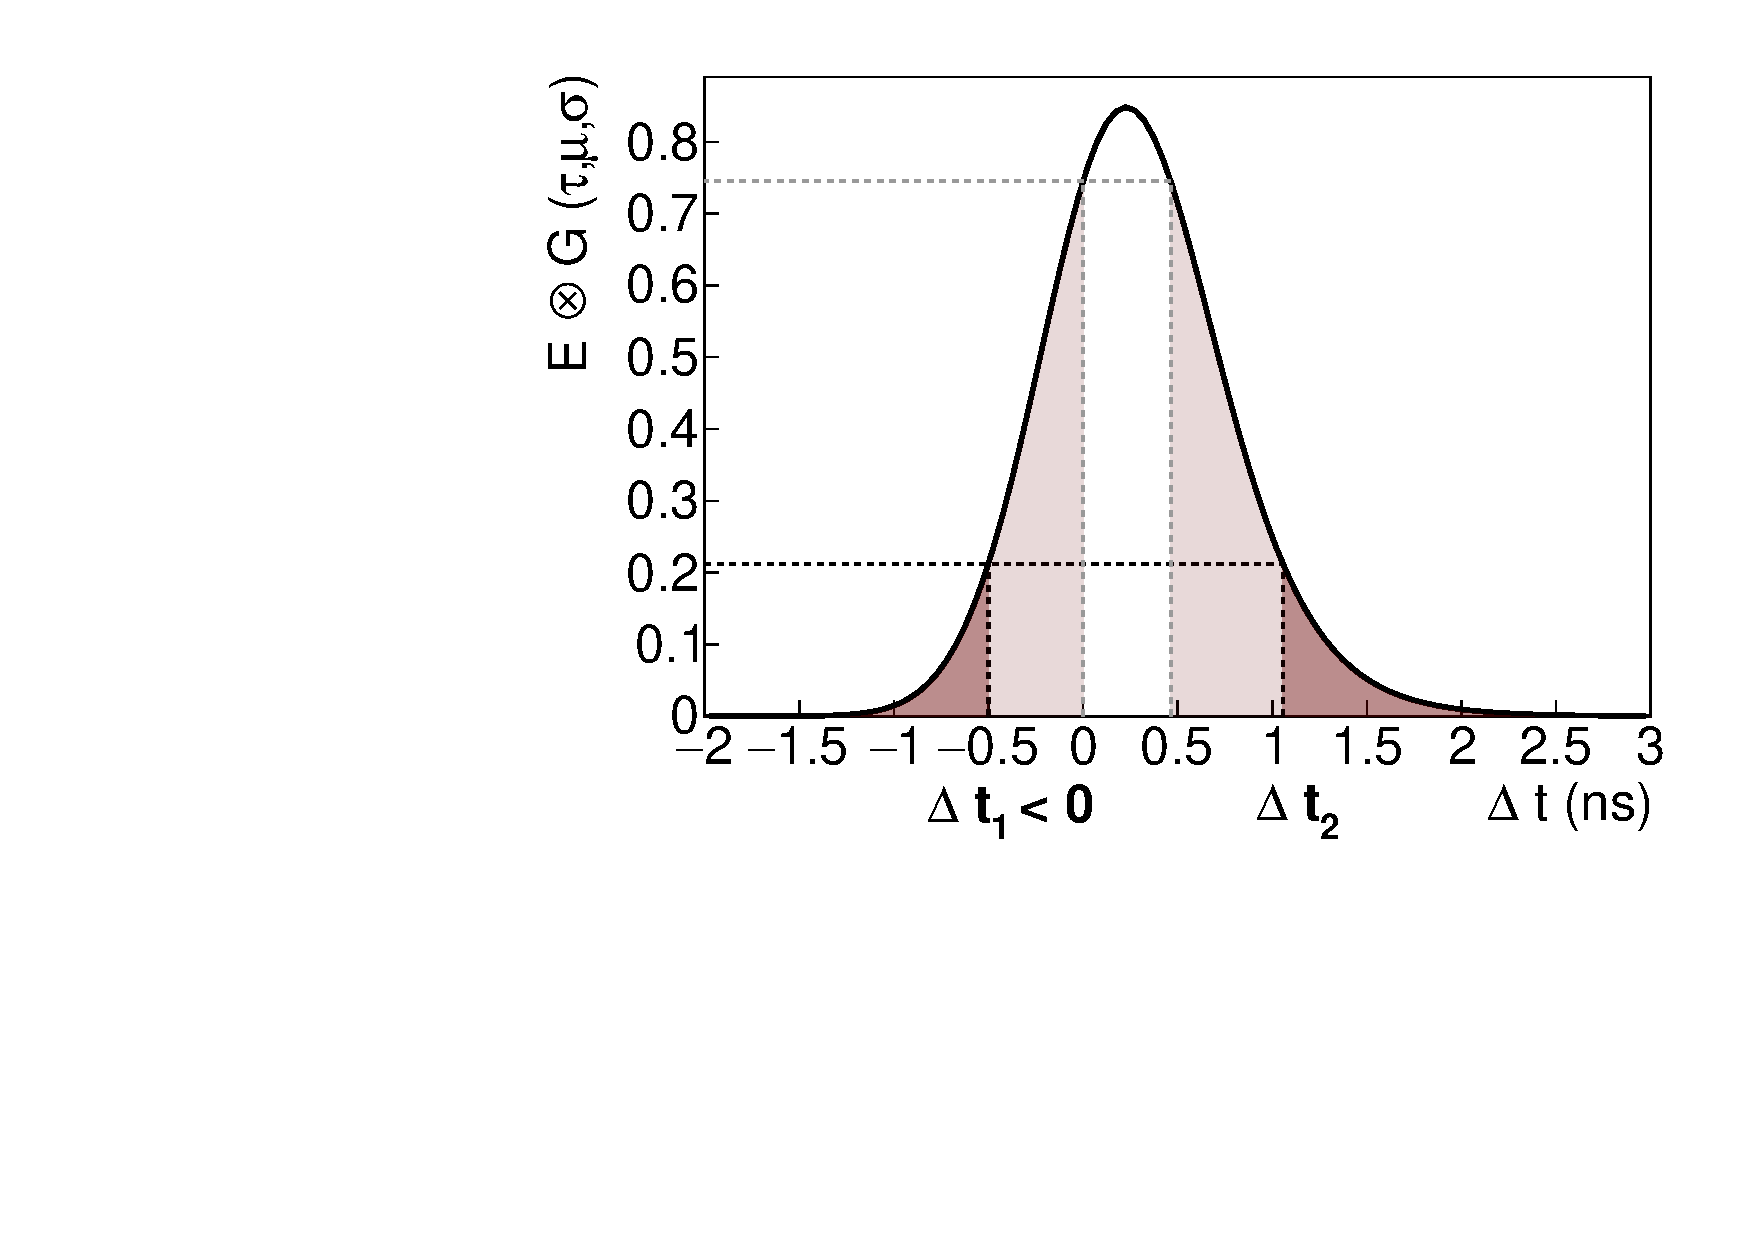
\includegraphics[width=0.64\textwidth]{timedifference/fig_timediff/proba_expo_1.pdf}
  \captionsetup{justification=justified}
  \caption{\Pint$\in[0;1]$ and $P_{exp}\in[0;0.65]$, with \Pint$>P_{exp}$
    \label{subfig:Proba_cut_1}}
\end{subfigure}
\vskip\baselineskip
\begin{subfigure}[t]{0.95\textwidth}
  \centering
  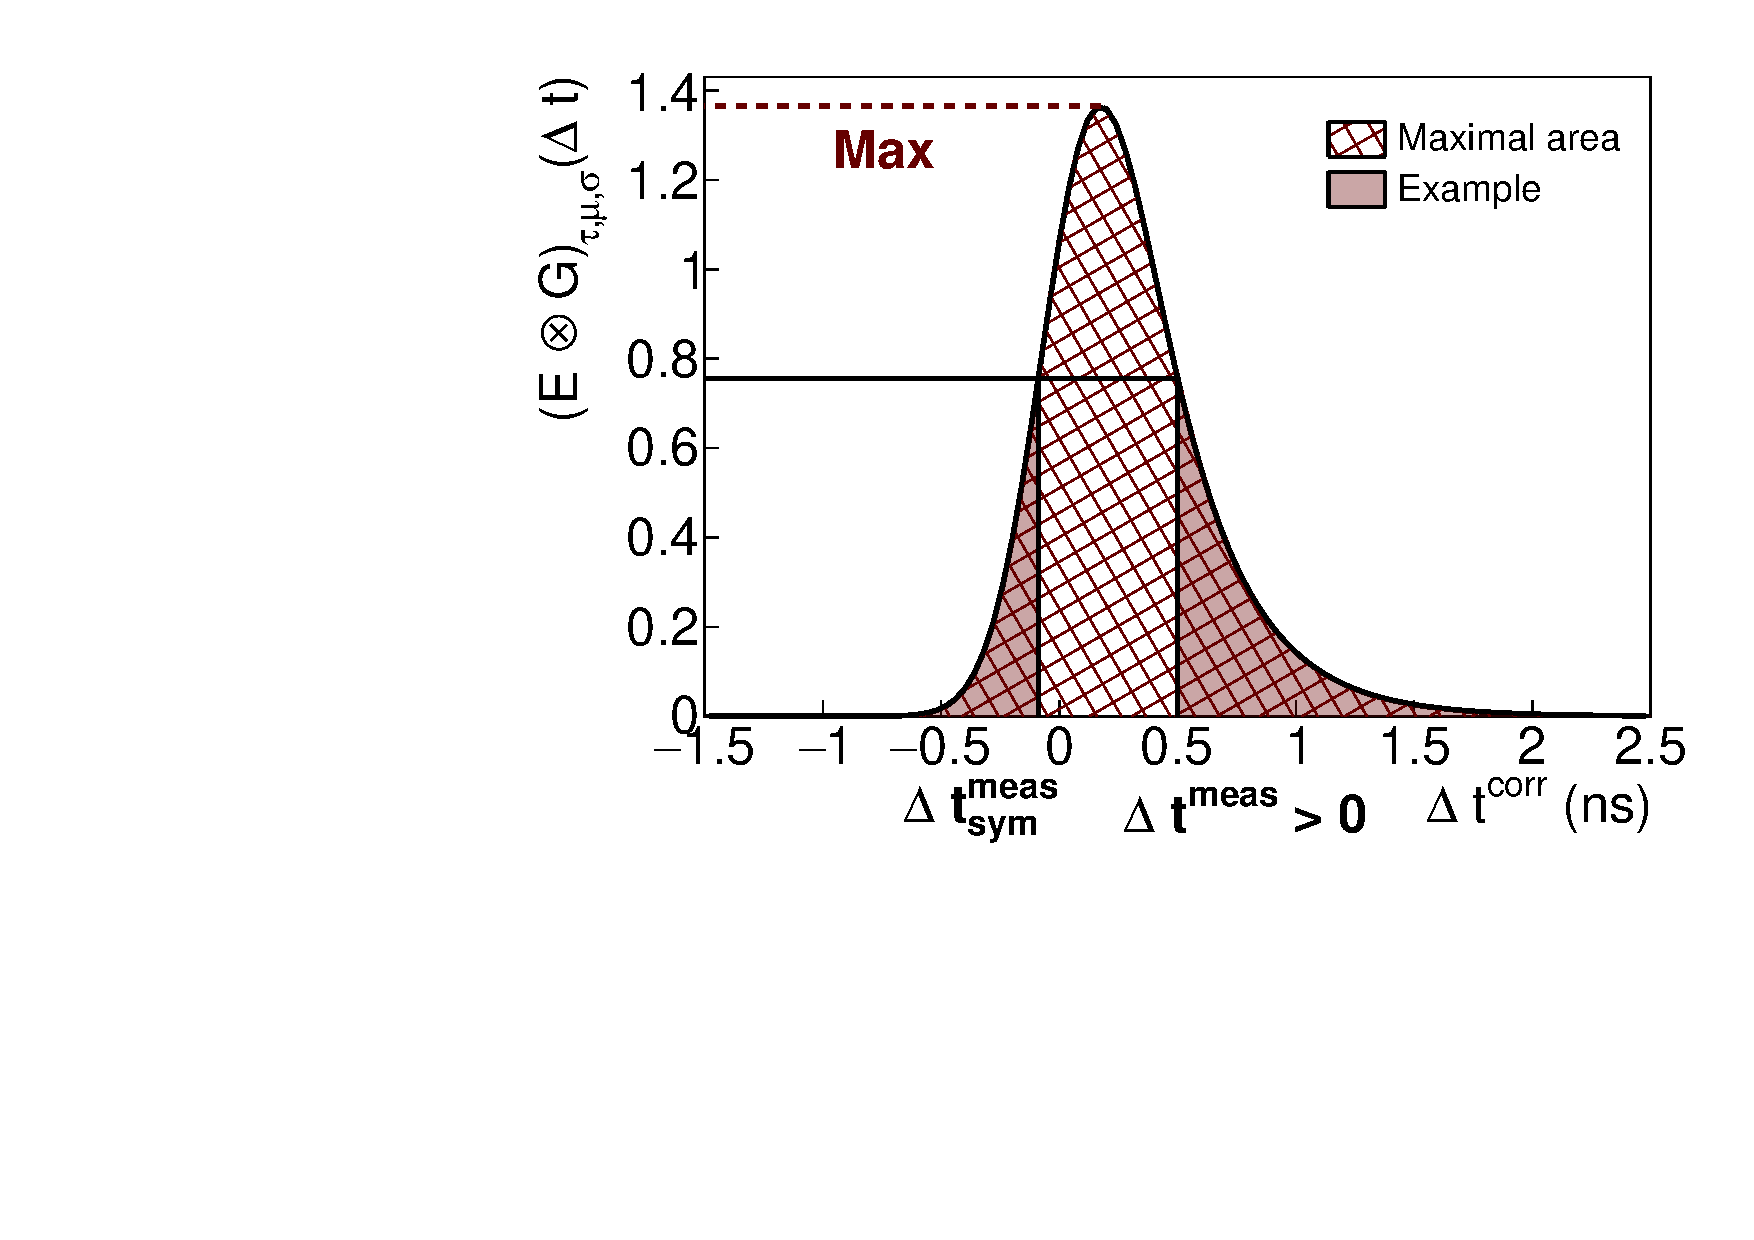
\includegraphics[width=0.64\textwidth]{timedifference/fig_timediff/proba_expo_2.pdf}
  \captionsetup{justification=justified}
  \caption{\Pint$\in[0;0.65]$ and $P_{exp}\in[0;1]$, with $P_{exp}>$\Pint
    \label{subfig:Proba_cut_2}}
\end{subfigure}
\vskip\baselineskip
\begin{subfigure}[t]{0.95\textwidth}
  \centering
  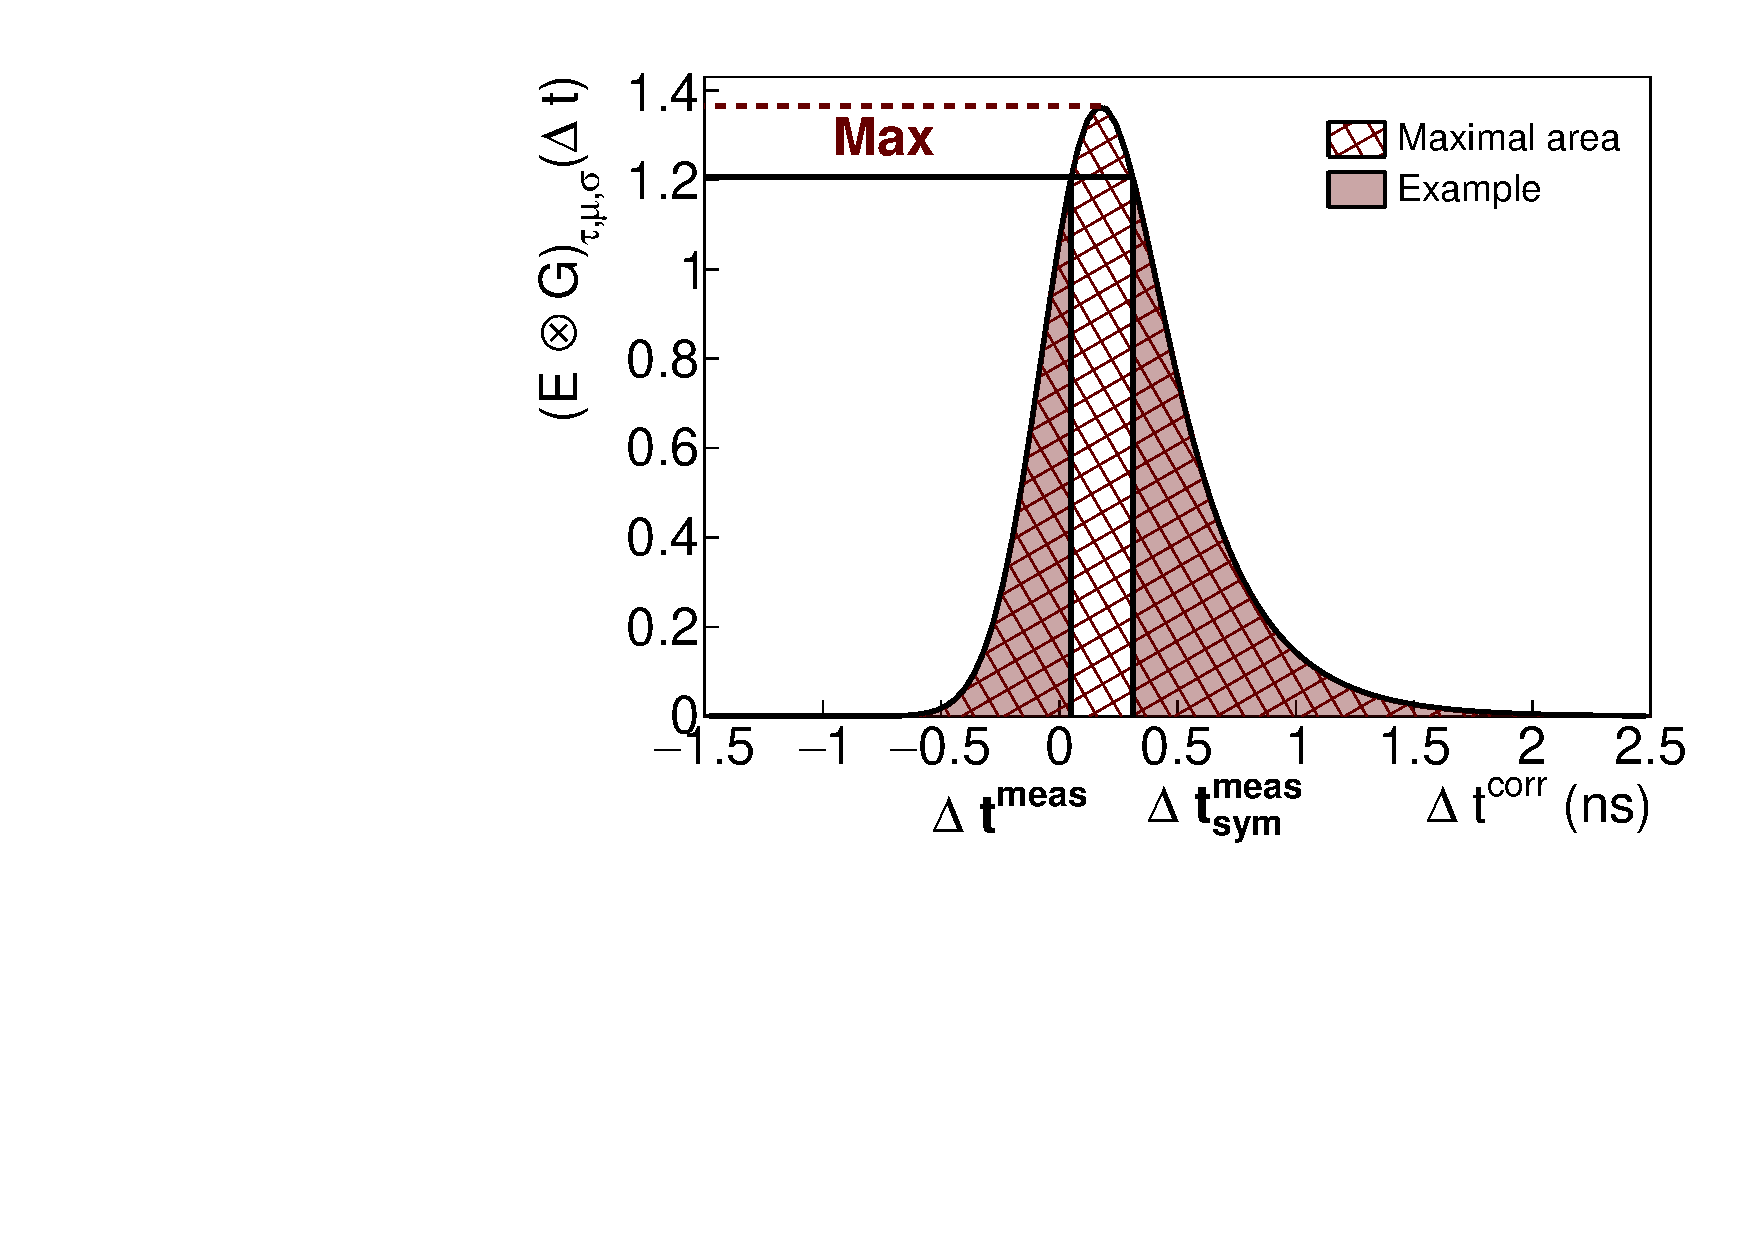
\includegraphics[width=0.64\textwidth]{timedifference/fig_timediff/proba_expo_3.pdf}
  \captionsetup{justification=justified}
  \caption{\Pint$\in[0.65;1]$ and $P_{exp}\in[0.65;1]$
    \label{subfig:Proba_cut_3}}
\end{subfigure}
\caption{${(E \otimes G)_{\tau,\mu,\sigma}(\Delta t)}$ distributions discribing the three areas observed in Fig.~\ref{fig:biplot_Pexp_Pint}.
  (a) $\Delta t^{\text{corr}} \in~]-\infty;0]$.
  (b) $\Delta t^{\text{corr}} \in~]\Delta t_{max};+\infty]$.
  (c) $\Delta t^{\text{corr}} \in~]0;\Delta t_{max}]$.
  \label{fig:proba_cut_ex}}
\end{figure}
\begin{enumerate}
\item \Pint$\in[0;1]$ and $P_{exp}\in[0;0.65]$, with \Pint$>P_{exp}$ (Fig.~\ref{subfig:Proba_cut_1}):\\
  This region corresponds to events for which $\Delta t^{\text{corr}}<0$.
  As the internal $\chi^{2}_{int}$ distribution is symmetrical, such events can have a value of \Pint\ varying from $0$ to $1$.
  Small values of \Pint\ correspond to events with a large $\Delta t^{\text{corr}}$ in absolute value.
  Conversely, the exponential distribution is not centred in zero.
  Therefore, if we limit to events for which the time difference is negative, we reach an upper bound for the value of the integral ($0.65$ in that case).
  This bound directly depends on the variations of the exponential distribution, therefore on the $\sigma_{t}$ value applied.
\item \Pint$\in[0;0.65]$ and $P_{exp}\in[0;1]$, with $P_{exp}>$\Pint (Fig.~\ref{subfig:Proba_cut_2}):\\
  These events have positive values for $\Delta t^{\text{corr}}$, beyond the ${(E \otimes G)_{\tau,\mu,\sigma}(\Delta t)}$ distribution maximum.
  The smaller the value of \Pint, the lower the probability that both particles were emitted at the same time into the source.
  Besides, for values of $\Delta t^{\text{corr}}$ highly positives, the value of the exponential probability can reach high values, up to $1$.
  The larger the value of $\Delta t^{\text{corr}}$ in positives, the smaller the value of $P_{exp}$.
\item \Pint$\in[0.65;1]$ and $P_{exp}\in[0.65,1]$ (Fig.~\ref{subfig:Proba_cut_3}):\\
  This region is also populated by events for which $\Delta t^{\text{corr}}>0$.
  Unlike the previous case, these events have small $\Delta t^{\text{corr}}$ values, meaning below the maximum of the exponential distribution.
  Also, these events have high internal probability values, as the probability that these two particles were emitted simultaneously is high.
  In the same way as the first bullet, the value of $P_{exp}$ is bounded: the lower bound corresponds to the value of the integral when $\Delta t^{\text{corr}}=0$ (here $0.65$).
  Once again, this bound is deeply related to the value considered for $\sigma_{t}$.
  The exponential probability can be equal to $1$ when $\Delta t^{\text{corr}}$ reaches the maximum of the exponential distribution.
\end{enumerate}

As discussed, the exponential probability quantifies the likelyhood that two particles were emitted with a delay corresponding to the radioactive exponential decay with ${\tau=294}$~ps, taking into account the time of flight resolution.
Therefore, we are interested in rejecting events for which values of $P_{exp}$ are high compared with the \Pint\ values.
In that case, a simple selection allowing to descriminate signal $\zeronu$ from delayed \Tl\ event consist in rejecting $2e$ topologies for which $P_{exp}~>~$\Pint\ (this cut-off is pictured in Fig.~\ref{fig:biplot_Pexp_Pint} by a plain black line).
With the previous explanation, we understand that such a cut is strongly linked to the cut on $\Delta t^{\text{corr}}$ presented in the previous sub-section.
%% For $\sigma_{t}=200$~ps, we are able to reject $41$\% of \Tl, while selecting $60$\% of $\zeronu$ $2e$ topologies for which $E>2.7$~MeV.
%% Although we are able to keep more $\zeronu$ events with this probability cut-off than for the one on time-of-flight difference, it is less efficient in rejecting \Tl\ events.

We would like to refine the selection made on the events using the two probabilities.
Regarding the biplot presented in Fig.~\ref{fig:biplot_Pexp_Pint}, the goal is to reject events located in the area $3$ and a part of the events located in area $2$.
Therefore, a more adapted cut-off is to reject events for which ${P_{exp}>0.65}$.
For this selection and ${\sigma_{t}=200}$~ps, we reject $20$\% of \Tl\ and keep $84$\% of $\zeronu$ events.
The proportion of signal events kept with this selection is satisfying.
Nevetheless the efficiency of \Tl\ rejection is almost $4$ times lower than for the time-of-flight selection presented in Sec.~\ref{subsec:tof_cutoff}.


%%  0nu 46 Tl avec > 0.65


\begin{itemize}
\item The final goal is to find optimal cut-offs in order to maximise the $90$\% CL limit set on $\Tbeta$.
\item relier le point d'inflexion du biplot à ce que l'on voit sur la fig eff 0nu / rej Tl
\item Donner le nb d'ev rejeté sur le nb d'ev total, puis sur le nb d'ev retardés
\end{itemize}


\subsection{Influence of the calorimeter time resolution}
\label{subsec:calo_sigma}

We study in this subsection the influence of the calorimeter timing resolution on event selections, using the two cut-offs presented above.

In Sec.~\ref{subsec:} we presented rejection efficiencies for a ${\Delta t>0}$ selection, with ${\sigma_{t}=200}$~ps.
In Fig.~\ref{fig:eff_cut_delta_t_sigma} is presented the $\zeronu$ selection efficiency with the rejection efficiency of \Tl, for values of $\sigma_{t}$ running from the ideal $0$~ps, to $400$~ps.
Each point corresponds to

As discussed, the variations of \Pint\ and $P_{exp}$ are binded to the value of $\sigma_{t}$, thus the levels applied on \Pint\ and $P_{exp}$ must be adapted to match these variations.


During the calorimeter R\&D, a great effort has been made to improve the optical modules energy resolution compared to Nemo-$3$, notably because it allows to have a better background rejection, and thus to decrease its contribution to the $\zeronu$ search.
Nevertheless, when it concerns background rejection, and especially the identification of $\beta$+IC delayed \Tl\ decays,


\begin{figure}[!h]
  \centering
  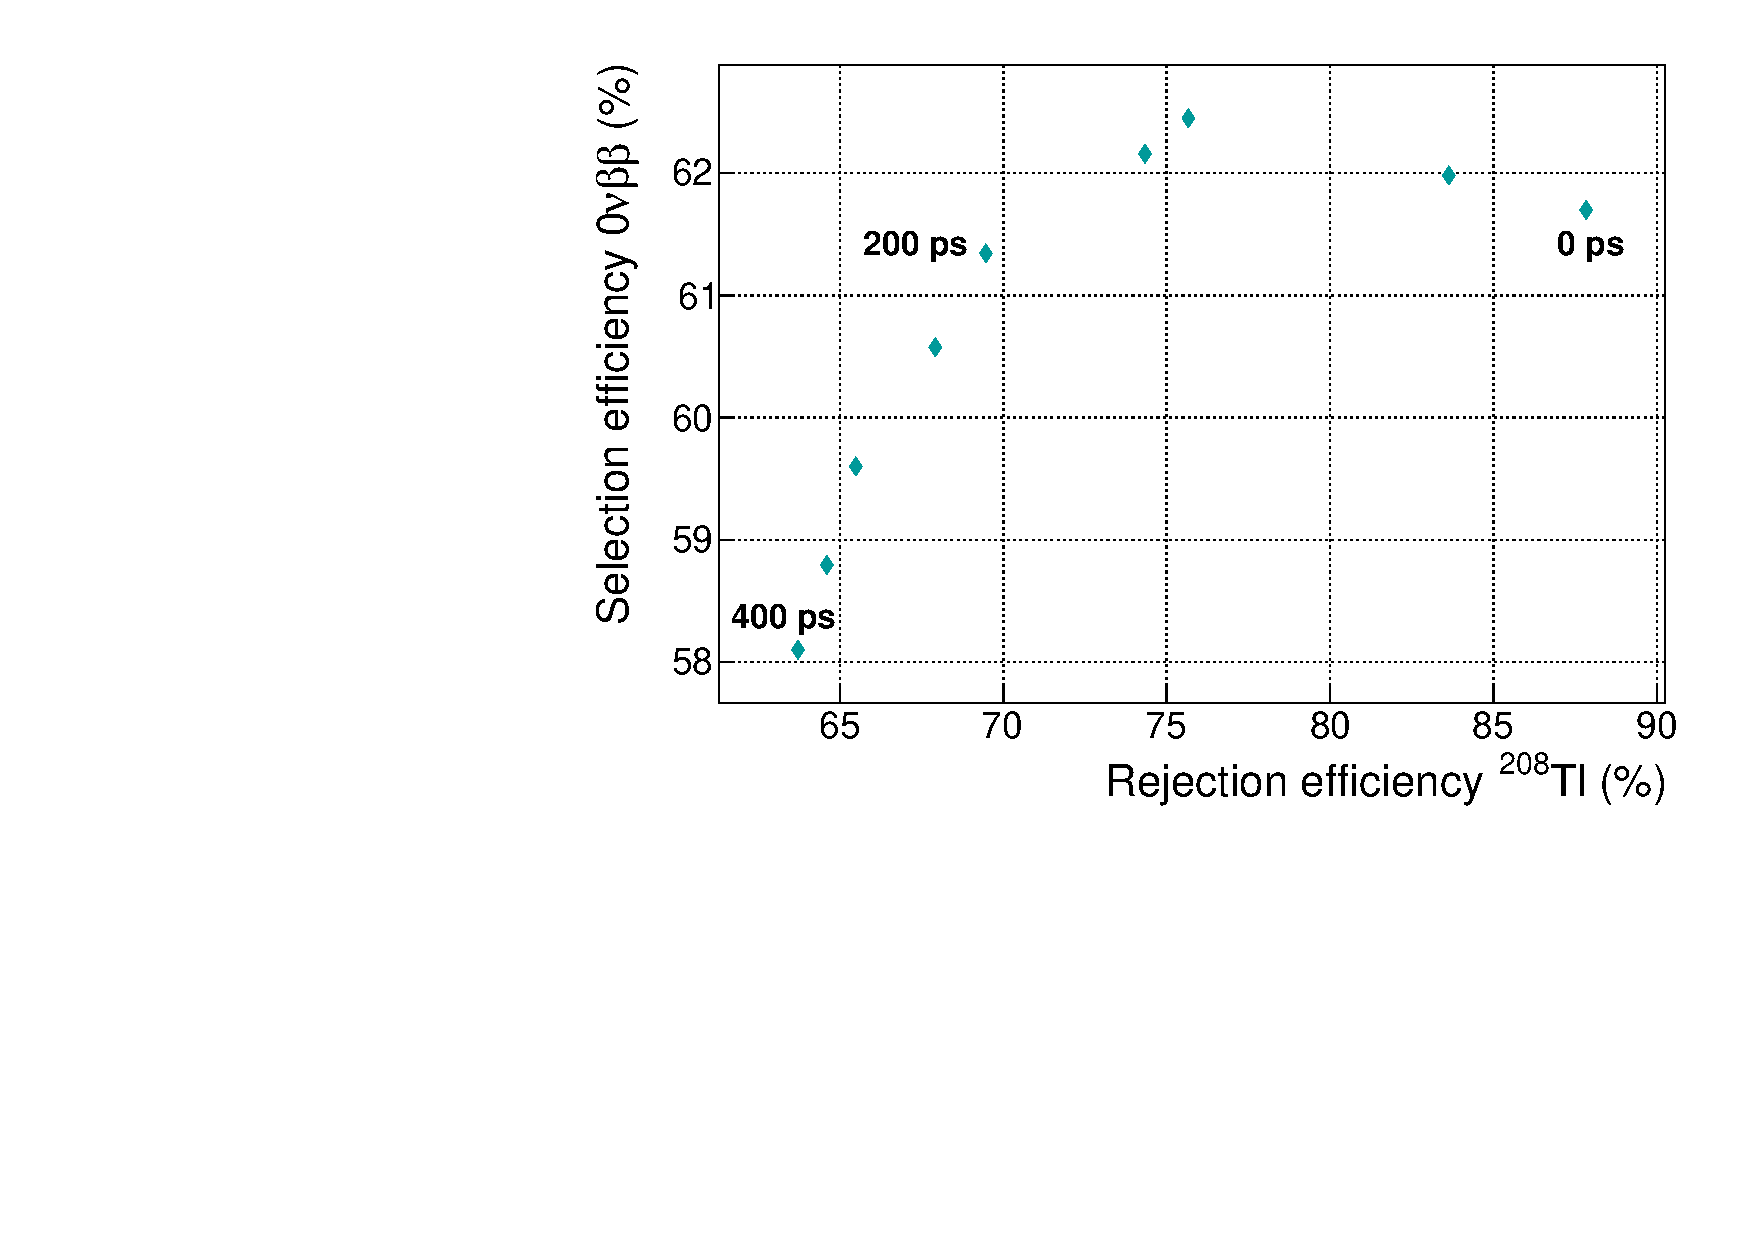
\includegraphics[width=13cm]{timedifference/fig_timediff/efficiency_proba.pdf}
  \caption{$\zeronu$ selection efficiency as a function of \Tl\ rejection.
    Each data point corresponds to a given value of $\sigma_{t}$, decrementing in $50$~ps steps.
    First order selections applied on $\zeronu$ and \Tl\ simulations.
    $\sigma_{l}=27.8$~ps.
    \label{fig:eff_proba_sigma}}
\end{figure}

\begin{figure}[!h]
  \centering
  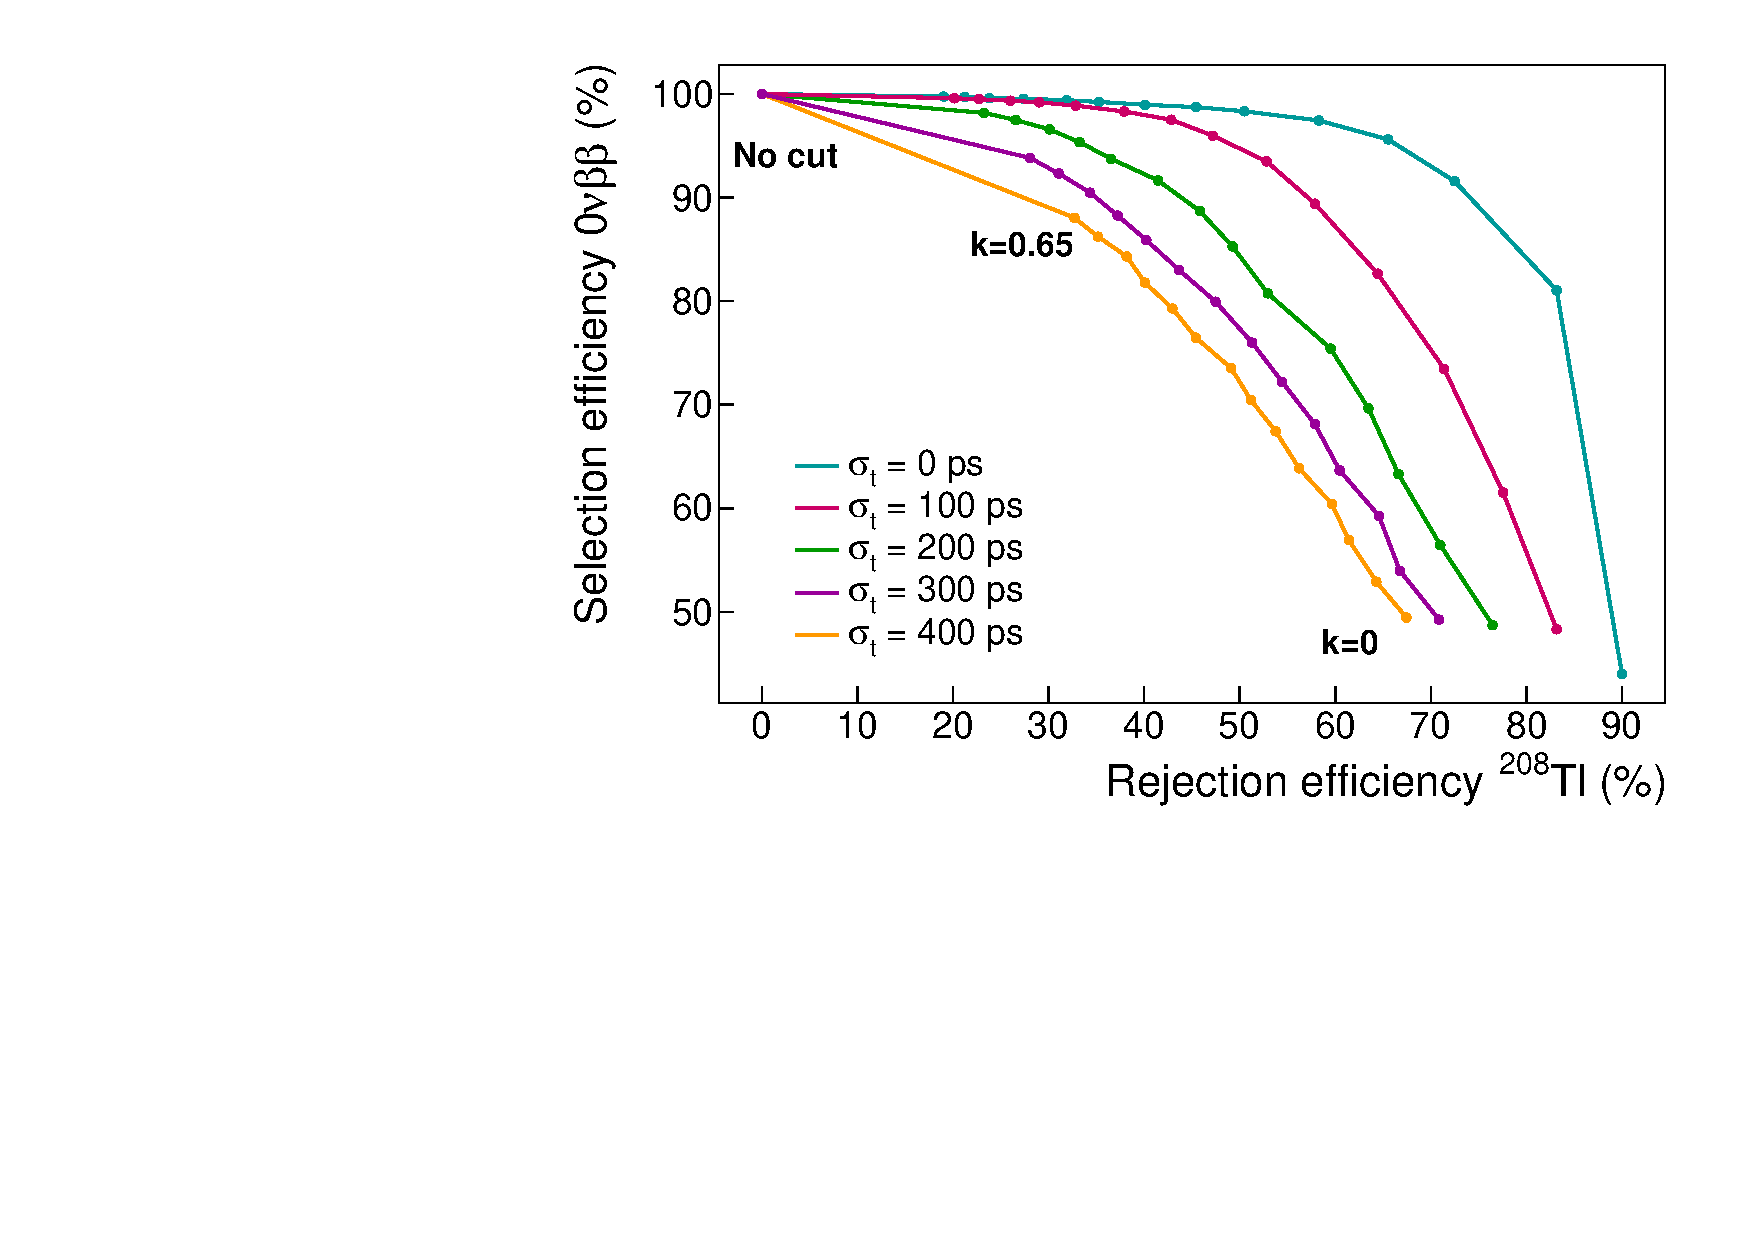
\includegraphics[width=13cm]{timedifference/fig_timediff/compare_sigma_cut_delta_t.pdf}
  \caption{$\zeronu$ selection efficiency as a function of \Tl\ rejection.
    Each curve corresponds to a given value of $\sigma_{t}$.
    Each data point corresponds to a minimum value for $\Delta t$.
    First order selections are applied on $\zeronu$ and \Tl\ simulations.
    $\sigma_{l}=27.8$~ps.
    \label{fig:eff_cut_delta_t_sigma}}
\end{figure}



\begin{figure}[!h]
  \centering
  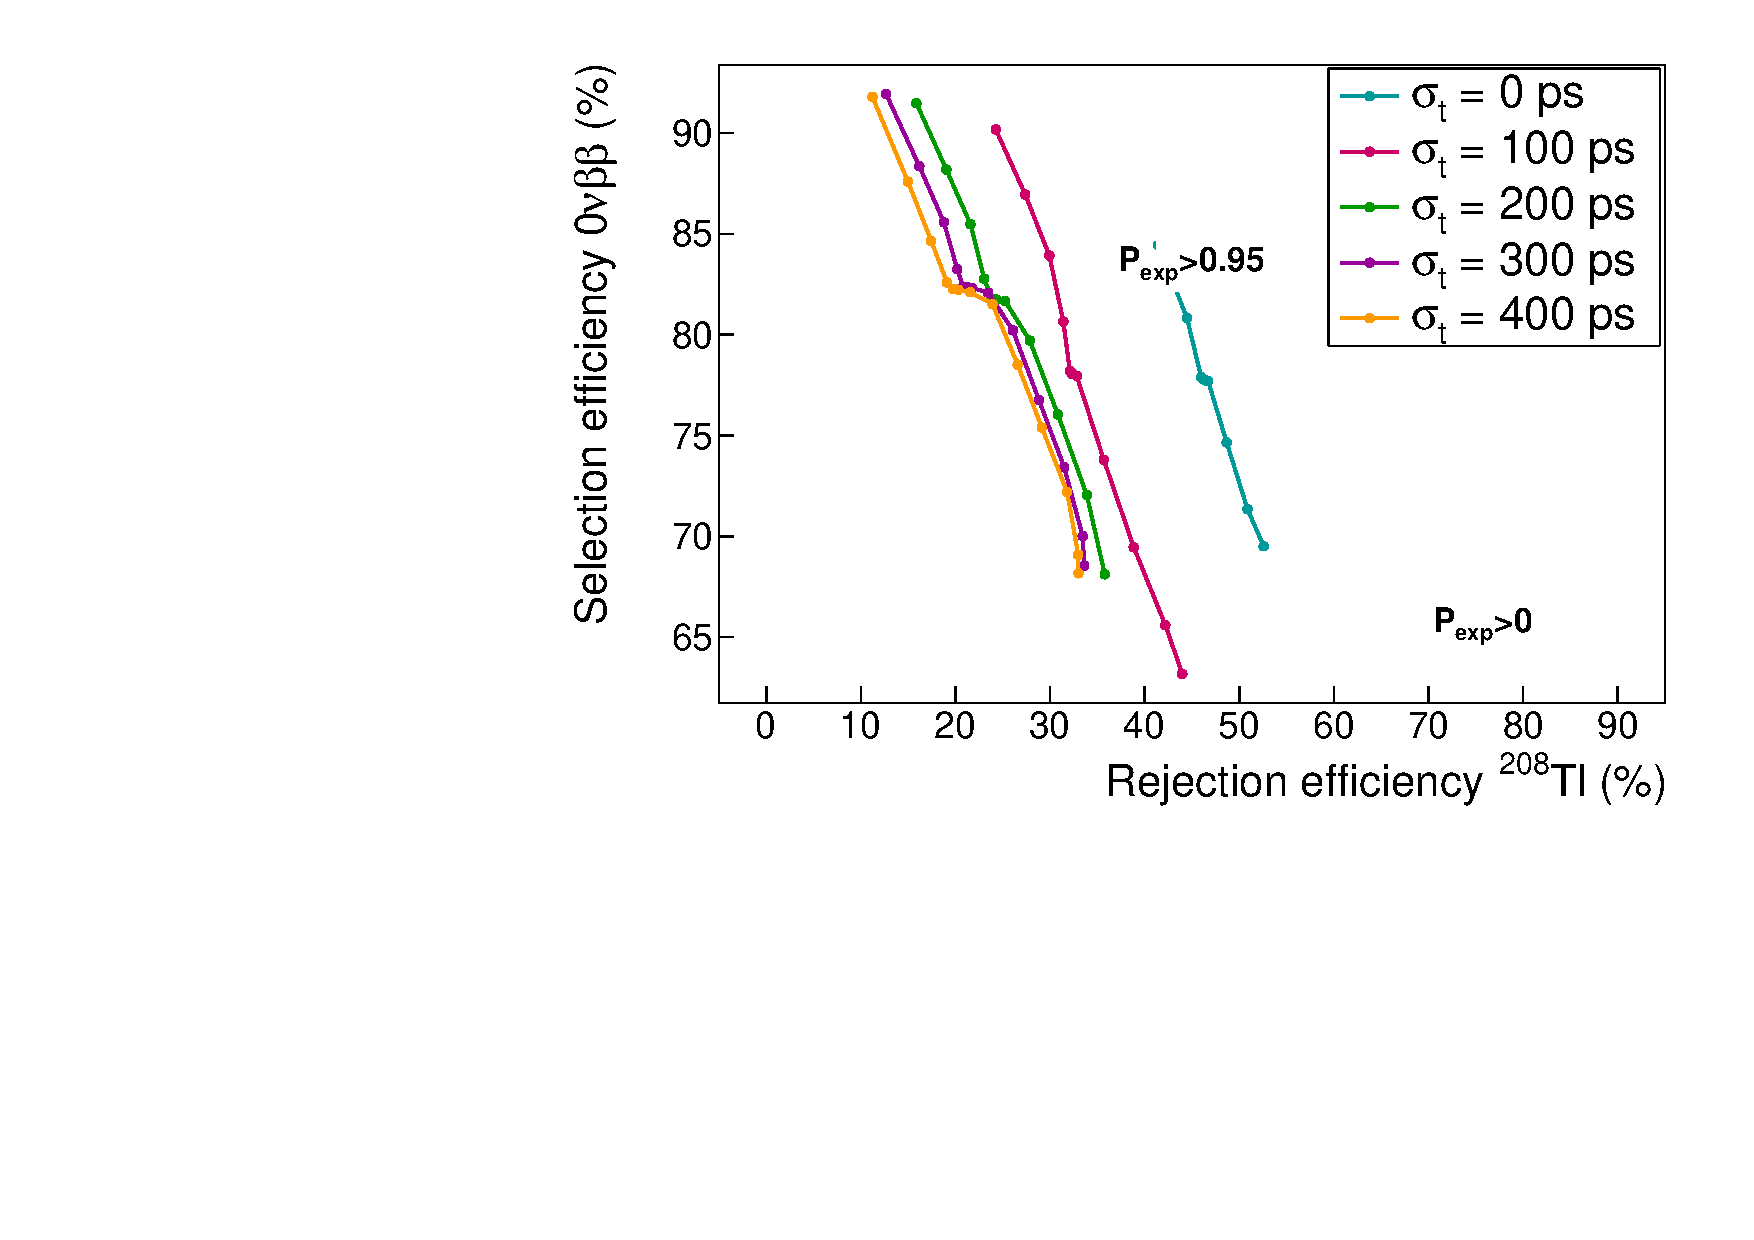
\includegraphics[width=13cm]{timedifference/fig_timediff/compare_sigma_cut_proba.pdf}
  \caption{$\zeronu$ selection efficiency as a function of \Tl\ rejection.
    Each data point corresponds to a given value of $\sigma_{t}$, decrementing in $50$~ps steps.
    First order selections applied on $\zeronu$ and \Tl\ simulations.
    $\sigma_{l}=27.8$~ps.
    \label{fig:eff_cut_proba_sigma}}
\end{figure}



\section{Impact of \Tl\ rejection on the experiment's sensitivity}
Reprendre l'analyse de sensibilité faite avec Axel en rajoutant les cuts Pint/Pexp et delta t pour le final detector

\begin{itemize}
\item cut efficiencies (delta t et proba) on other backgrounds
\item Se servir des résultats de $\sigma_{t}$ trouvés au chap.~\ref{chap:Cobalt_study}
\item Mais dire que ces sigmas peuvent être améliorés
\item donc présenter l'évolution des résultats (efficacité de réjection et sensibilité) sur la réjection en fonction de la valeur de sigma t, à faire varier dans un certain range.
\item Tu pourrais avec une figure à 2D où tu montres l'efficacité relative 0nu (égale à 100\% avant cette coupure temporelle) en fonction de la réjection du Tl208 -> cela donne une courbe que tu parcoures et tu cherches à optimiser ton point de fonctionnement.
\item Peut-être que quand tu commenteras la courbe tu pourras insister sur le rôle très important de l'amélioration de sigma t, en donnant des chiffres pour une efficacité 0nu fixée (par exemple à 95\%), voir quelle serait la réjection du Tl208 pour sigma t = 400 ps, 200ps, 100 ps.
\end{itemize}


\section{Conclusion}

\begin{itemize}
\item On peut éventuellement mettre une source de 232U dans le détecteur (un des parents de 208Tl) pour tester la réjection.
\item ajout sélection énergie
\item plus correct de couper sur Pexp que sur delta t car on tient compte des erreurs
Improving the time resolution of the calorimeter is not the purpose of the R\&D programme, however it has benefited from the high light output achieved to meet the energy resolution goals.
The time resolution of the optical modules has been monitored at every stage of the R\&D programme.

\end{itemize}


\begin{figure}[!h]
  \centering
  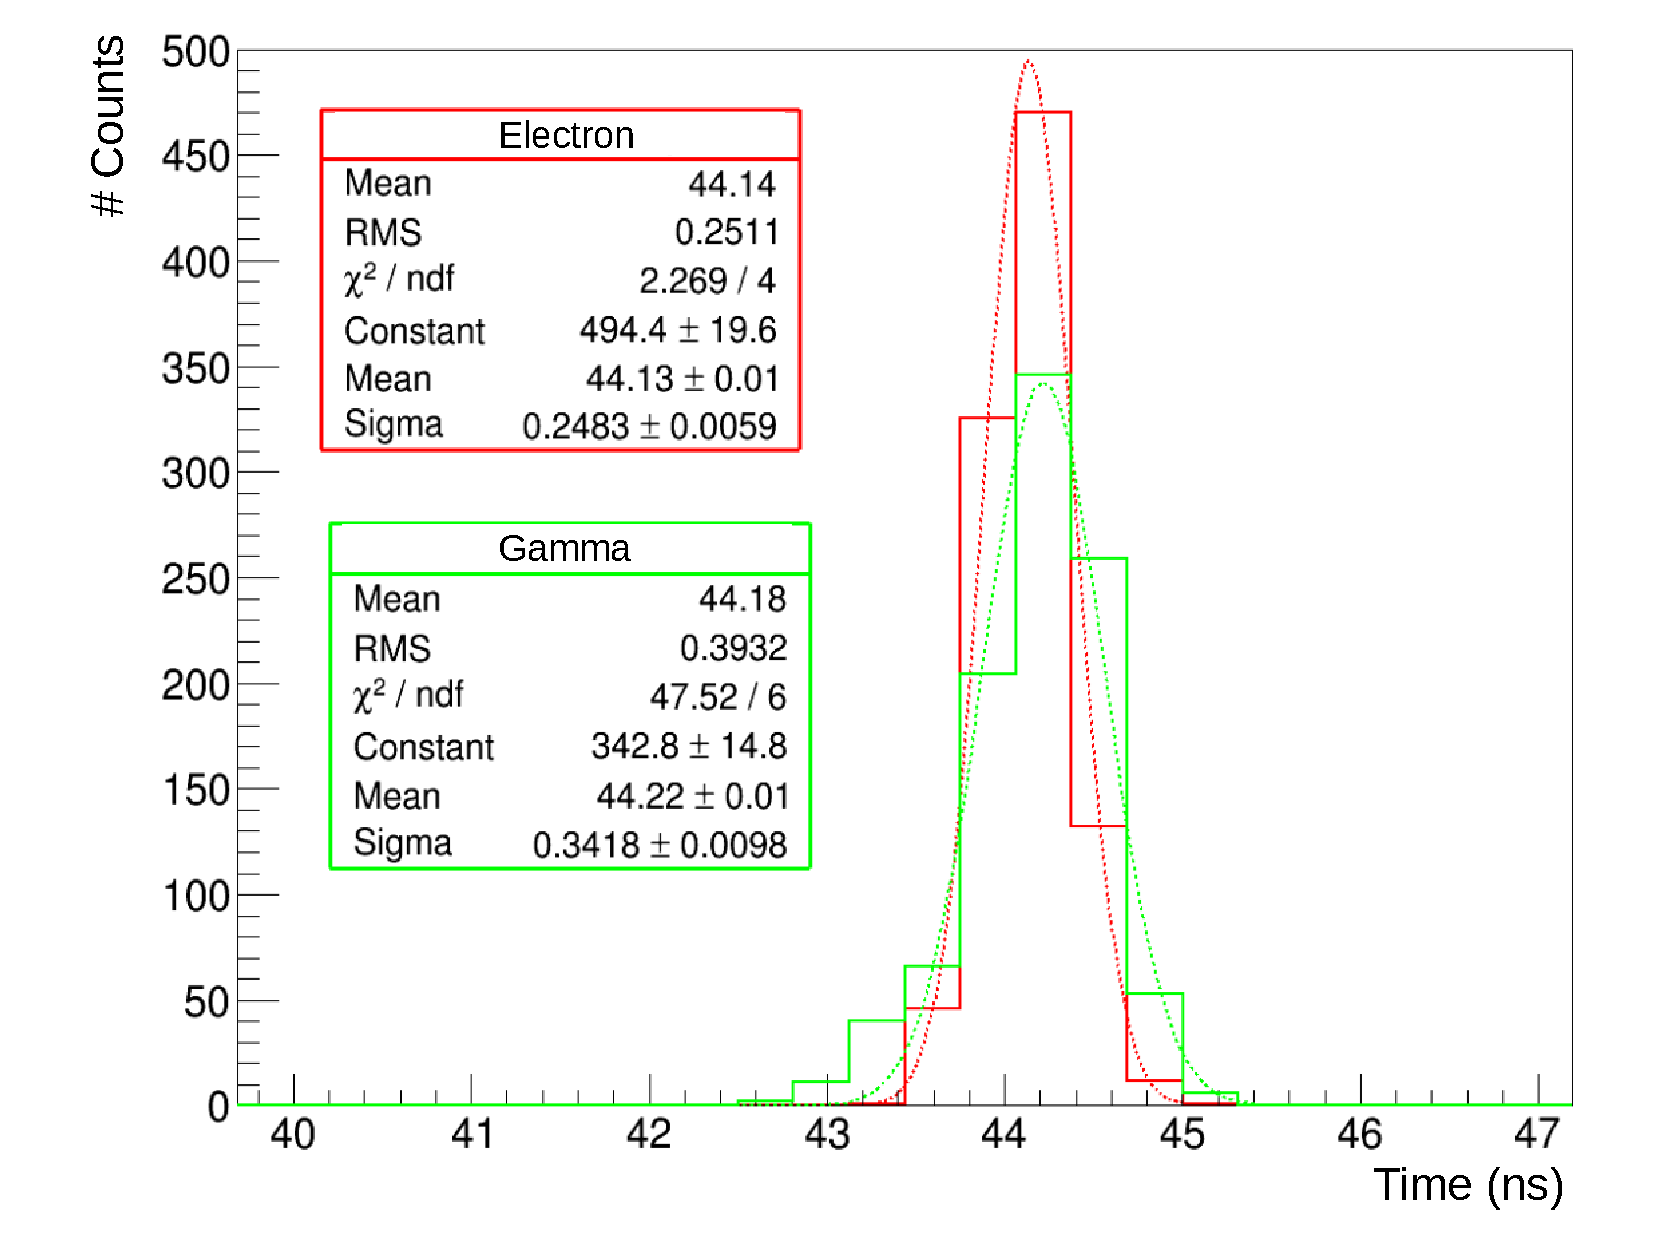
\includegraphics[width=13cm]{timedifference/fig_timediff/Arnaud_RMS_PM.pdf}
  \caption{Time distribution of the trigger time of an optical module in the case of electrons (red) and gamma radiation (green) depositing an energy of $1$~MeV in the scintillator.
    The trigger threshold is set at $45$ mV and corresponds to an energy of $0.150$~MeV.
    Adapted from~\cite{HuberThesis}.
  \label{fig:Arnaud_RMS_PM}}
\end{figure}
